% main_unificado.tex -- Datos clínicos y modelización descriptiva
% Curso de Verano 2026, Universidad de Cantabria
% 43 diapositivas, ~50 minutos
% Compilar: pdflatex main_unificado.tex (dos veces para referencias cruzadas)
% Imágenes en ../plots/
%
% ESTRUCTURA (50 min, pausa a criterio del ponente):
%   Apertura        slides  1- 2  (portada, visión general)
%   Bloque 1        slides  3-14  (datos clínicos)
%   Bloque 2        slides 15-28  (estadística descriptiva)
%   Bloque 3        slides 29-38  (visualización)
%   Cierre          slides 39-43
% -------------------------------------------------------------------------
\documentclass[aspectratio=169,10pt]{beamer}
% Pacotes
\usepackage{lipsum}
\usepackage{graphicx}
\usepackage{color}
\usepackage[table]{xcolor}
\usepackage{tikz}
\usepackage{tcolorbox}
\usepackage{amsmath}
\usepackage{amsfonts}
\usepackage{amssymb}
\usepackage{mathrsfs}
\usepackage{mathtools}
\usepackage{enumitem} 
\usepackage{float}
\usepackage[utf8]{inputenc}	

\usepackage{caption}

\usepackage[spanish, es-tabla]{babel}
\usepackage[babel, spanish=spanish]{csquotes}
\AtBeginEnvironment{quote}{\small}
\decimalpoint

\usetikzlibrary{decorations.pathreplacing,calc}
\usetikzlibrary{shadows}
\usetikzlibrary{positioning}

\usepackage{booktabs}

\usepackage{subcaption}

\usepackage{multicol}

\usepackage{multirow}


% Theme choice:
\usetheme{CambridgeUS}

% Cores personalizadas
\definecolor{PROFMATgreen}{RGB}{0, 138, 163}
\definecolor{UFTgreen}{RGB}{0, 137, 124}
\definecolor{UFTblue}{RGB}{0, 84, 132}
\definecolor{UFTyellow}{RGB}{253, 185, 46}
\definecolor{UFTgray}{RGB}{132, 134, 136}

\definecolor{UC}{RGB}{0,178,169}

% Ativar numeração de tabelas
\setbeamertemplate{caption}[numbered]

% Definir novo estilo de item com quadrado verde
\setlist[itemize,1]{label=\textcolor{UFTgreen}{\rule{1ex}{1ex}}}

\setbeamercolor*{structure}{bg=UFTgreen,fg=black}

\setbeamercolor*{palette primary}{fg=black,bg=PROFMATgreen}
\setbeamercolor*{palette secondary}{fg=white,bg=UFTblue}
\setbeamercolor*{palette tertiary}{fg=black,bg=UFTgreen}
\setbeamercolor*{palette quaternary}{fg=white,bg=black}

\setbeamercolor{section in toc}{fg=black,bg=white}
\setbeamercolor{alerted text}{fg=white}

\setbeamercolor*{item}{fg=PROFMATgreen}

\setbeamercolor{block title}{bg=UFTgreen,fg=white}
\setbeamercolor{block body}{bg=UFTgray!10,fg=black}

\setbeamercolor{titlelike}{fg=white, bg=UFTblue}
\setbeamercolor{frametitle}{bg=UFTgray!20,fg=UFTgreen}



\setbeamertemplate{background}{
    \parbox[c][\paperheight][c]{\paperwidth}{
        \vfill
        
\includegraphics[width=\paperwidth,height=\paperheight,keepaspectratio]{img/modelo/bakcground.png} 
        \vfill
    }
}


% Personalizar portada
\setbeamertemplate{title page}{
  \begin{columns}[c,totalwidth=\paperwidth]
    \column{.05\paperwidth}
      \centering
      \raisebox{0.1cm}{%
        \parbox{.5\paperwidth}{\centering\scriptsize
        Cursos de Verano\\
        LA 2.4 Inteligencia Artificial en Estudios Clínicos\\
        Laredo, Cantabria · 1 -- 3 julio 2026}
      }
    \column{.45\paperwidth}
      \centering
      
\includegraphics[height=1.2cm]{img/UC_LogotipoPrincipal.png}
\end{columns}

  \vskip1em
  \begingroup
    \centering
    \begin{beamercolorbox}[sep=8pt,center,shadow=true,rounded=false]{title}
      \usebeamerfont{title}\inserttitle\par%
      \ifx\insertsubtitle\@empty\else
        \vskip0.25em{\usebeamerfont{subtitle}\usebeamercolor[fg]{subtitle}\insertsubtitle\par}%
      \fi
    \end{beamercolorbox}
    \vskip1em
    \begin{beamercolorbox}[sep=6pt,center]{author}\usebeamerfont{author}\insertauthor\end{beamercolorbox}
    \vskip0.2em
    \begin{beamercolorbox}[sep=5pt,center]{advisor}\usebeamerfont{institute}\advisorname\end{beamercolorbox}
    \vskip0.2em
    \begin{beamercolorbox}[sep=5pt,center]{institute}\usebeamerfont{institute}\insertinstitute\end{beamercolorbox}
    \vskip0.2em
    \begin{beamercolorbox}[sep=5pt,center]{date}\usebeamerfont{institute}\insertdate\end{beamercolorbox}
    \vskip0.5em
  \endgroup
  \vfill
}



% Remover bordas arredondadas dos blocks
\makeatletter
\setbeamertemplate{blocks}[default] % Isso remove o arredondamento
\makeatother


% Pacotes de citações
% ---

\usepackage[alf,abnt-etal-text=it,abnt-repeated-author-omit=yes,abnt-etal-list=0,abnt-etal-cite=3,abnt-emphasize=bf]{abntex2cite}	% Citações padrão ABNT



\setbeamercolor{bibliography entry author}{fg=black}
\setbeamertemplate{bibliography item}{\newblock}


\setbeamertemplate{frametitle continuation}{}

% Redefinir o separador para um traço
% Redefinir o separador
\captionsetup[figure]{labelformat=simple, labelsep=endash, textformat=period, font=footnotesize}
\captionsetup[table]{labelformat=simple, labelsep=endash, textformat=period, font=footnotesize}


% Redefine espaçamento antes e depois da legenda em figuras e tabelas
\captionsetup[figure]{aboveskip=2pt, belowskip=0pt}
\captionsetup[table]{aboveskip=2pt, belowskip=0pt}


% Define uma penalidade alta para a hifenização
\hyphenpenalty=10000
\tolerance=10000


% Personalizando o estilo da tabela de conteúdos
\setbeamertemplate{section in toc}[sections numbered]
\renewcommand{\thesection}{\textcolor{PROFMATgreen}{\arabic{section}}}
\renewcommand{\thesubsection}{\textcolor{PROFMATgreen}{\arabic{section}.\arabic{subsection}}}

\setbeamersize{text margin left=0.8cm, text margin right=0.8cm}


% ── Alias de colores (UC* → paleta UFT de customizacoes) ─────────────────────
\colorlet{UCblue}     {UFTblue}
\colorlet{UCblueLight}{PROFMATgreen}
\colorlet{UCbluePale} {UFTblue!15}
\colorlet{UCgreen}    {UFTgreen}
\colorlet{UCgray}     {UFTgray}
\definecolor{UCred}   {RGB}{180,30,30}
\definecolor{UCorange}{RGB}{210,100,0}
% ── \advisorname requerido por customizacoes.tex ─────────────────────────────
\newcommand{\advisorname}{}
\setbeamercolor{advisor}{fg=black}
% ── Ruta de imágenes ─────────────────────────────────────────────────────────
\graphicspath{{../plots/}{./}}
% ── Imagen con placeholder (sin nombre de fichero para evitar _ en texto) ────
\newcommand{\maybeincludegraphics}[2][width=\textwidth]{%
  \IfFileExists{../plots/#2}%
    {\includegraphics[#1]{#2}}%
    {\parbox[c][3cm][c]{\linewidth}{\centering\textcolor{UFTgray}{\tiny[imagen pendiente]}}}%
}

\newcommand{\yes}{\textcolor{UCgreen!70!black}{\checkmark}}
\newcommand{\no}{\textcolor{UCred}{$\boldsymbol{\times}$}}

\title[Datos clínicos y modelización descriptiva]{Datos Clínicos y Modelización Descriptiva}
\subtitle{Calidad del dato, estadística descriptiva y visualización\\para investigadores clínicos}
\author[Diego García-Prieto]{%
  Diego García-Prieto\\[1mm]
  {\small\texttt{diego.garciaprieto@unican.es}}}
\institute[UC]{Dpto.\ Matemáticas, Estadística y Computación \\Universidad de Cantabria}
\date{2 de julio de 2026}

% =========================================================================
\begin{document}
% =========================================================================


% =========================================================================
% APERTURA
% =========================================================================

% SLIDE 1 - Portada -------------------------------------------------------
\begin{frame}
  \titlepage
\end{frame}

% SLIDE 2 - Sesión en un vistazo -------------------------------------------
\begin{frame}{Esta sesión en un vistazo}
  \begin{columns}[T]
    \begin{column}{0.50\textwidth}
      \begin{block}{Contenido}
        \begin{enumerate}\small
          \item[\textbf{1.}] ¿Qué es un dato clínico?\\
                \scriptsize Tipos · Outliers · Sesgos · Missings
          \vspace{2mm}
          \item[\textbf{2.}] Estadística descriptiva\\
                \scriptsize Table~1 · Media/mediana · Correlaciones
          \vspace{2mm}
          \item[\textbf{3.}] Visualización\\
                \scriptsize Histogramas · Boxplots · Scatter · ROC
        \end{enumerate}
      \end{block}
    \end{column}
    \begin{column}{0.47\textwidth}
      \begin{exampleblock}{Al terminar sabréis\ldots}
        \begin{enumerate}\small
          \item[\textbf{1.}] \textbf{Detectar} si vuestros datos\\
                son fiables
          \vspace{3mm}
          \item[\textbf{2.}] \textbf{Construir} el Table~1\\
                de cualquier artículo clínico
          \vspace{3mm}
          \item[\textbf{3.}] \textbf{Elegir} el gráfico correcto\\
                para cada situación
        \end{enumerate}
      \end{exampleblock}
    \end{column}
  \end{columns}
\end{frame}


% =========================================================================
\section{¿Qué es un dato clínico?}
% =========================================================================

% Separador bloque 1 -------------------------------------------------------
\begin{frame}[plain]
  \begin{center}
    \vspace{14mm}
    \begin{beamercolorbox}[sep=22pt,center,rounded=true,shadow=true]{block title}
      {\large Bloque 1}\\[4mm]
      \LARGE\bfseries ¿Qué es un dato clínico?
    \end{beamercolorbox}
    \vspace{8mm}
    {\large\color{UCgray} Tipos, calidad y trampas frecuentes.}
  \end{center}
\end{frame}

% SLIDE 4 - ¿Qué es un dato clínico? ----------------------------------------
\begin{frame}{¿Qué es un dato clínico?}
  \begin{columns}[T]
    \begin{column}{0.52\textwidth}
      \begin{block}{Definición}
        \small Cualquier \textbf{medición, observación o registro}\\
        generado en el contexto de la atención sanitaria.
        \vspace{3mm}
        \begin{itemize}\small
          \item Resultados de laboratorio, constantes vitales
          \item Diagnósticos, síntomas, tratamientos
          \item Tiempos de evento, escalas clínicas
        \end{itemize}
      \end{block}
      \vspace{3mm}
      \begin{block}{Se distingue de\ldots}
        \scriptsize
        \textbf{Dato experimental:} condiciones controladas de laboratorio\\[1mm]
        \textbf{Dato administrativo:} codificación, facturación, gestión
      \end{block}
    \end{column}
    \begin{column}{0.45\textwidth}
      \vspace{3mm}
      \begin{block}{Característica esencial}
        \small El dato clínico es \textbf{heterogéneo, ruidoso\\
        y con missings por naturaleza}.\\[2mm]
        \scriptsize No por descuido.\\
        Por la realidad de la práctica clínica diaria.
      \end{block}
      \vspace{3mm}
      \begin{exampleblock}{Fuentes habituales}
        \scriptsize
        Historia clínica electrónica (EHR)\\
        Sistemas REDCap / bases de datos ad hoc\\
        Registros de laboratorio e imagen\\
        Cuadernos de recogida de datos (CRD)
      \end{exampleblock}
    \end{column}
  \end{columns}
\end{frame}

% SLIDE 5 - El punto de partida -------------------------------------------
\begin{frame}{El punto de partida real: vuestros datos}
  \begin{columns}[T]
    \begin{column}{0.50\textwidth}
      \begin{block}{Lo que veis cuando abrís el REDCap del servicio}
        \begin{itemize}\small
          \item 200 variables; 40 sin saber por qué las pusisteis
          \item Una columna llamada \texttt{Dato2} que nadie sabe qué es
          \item Valores imposibles: glucosa\,=\,0\,mg/dL
          \item Fechas que no cuadran: alta antes del ingreso
          \item 30\,\% de missings en la variable que más necesitáis
        \end{itemize}
      \end{block}
      \vspace{3mm}
      \begin{block}{}
        \scriptsize Esto no es un dataset limpio de Kaggle.\\
        Es la realidad de cualquier servicio clínico.
      \end{block}
    \end{column}
    \begin{column}{0.47\textwidth}
      \centering\vspace{2mm}
      \begin{tikzpicture}[scale=0.72,transform shape]
        \fill[UCblue!80] (0,3.6) rectangle (6.0,4.2);
        \node[right,font=\tiny\bfseries,text=white] at (0.08,3.88)
          {ID\enspace Glucosa\enspace Peso\enspace Dato2\enspace Fecha\_alta};
        \fill[UCbluePale] (0,3.0) rectangle (6.0,3.5);
        \node[right,font=\tiny] at (0.08,3.22)
          {001\enspace 120\enspace\quad 72.3\enspace 37.2\enspace 12/03/2024};
        \fill[UCred!14] (0,2.4) rectangle (6.0,2.9);
        \node[right,font=\tiny] at (0.08,2.62)
          {002\enspace \textcolor{UCred}{\bfseries 0}\enspace\quad\; 68.1\enspace 36.9\enspace 15/03/2024};
        \fill[UCbluePale] (0,1.8) rectangle (6.0,2.3);
        \node[right,font=\tiny] at (0.08,2.02)
          {003\enspace 115\enspace\quad ---\enspace\;\; \textcolor{UCred}{\bfseries ?}\enspace\;\; 18/03/2024};
        \fill[UCred!14] (0,1.2) rectangle (6.0,1.7);
        \node[right,font=\tiny] at (0.08,1.42)
          {004\enspace 98\enspace\quad\; 81.0\enspace 37.0\enspace \textcolor{UCred}{\bfseries 01/01/2024}};
        \fill[UCbluePale] (0,0.6) rectangle (6.0,1.1);
        \node[right,font=\tiny] at (0.08,0.82)
          {005\enspace ---\enspace\quad ---\enspace\;\; ---\enspace\;\; ---};
        \draw[UCblue!40,thin] (0,0.6) rectangle (6.0,4.2);
      \end{tikzpicture}
      \vspace{1mm}\\
      {\scriptsize\color{UCgray} Glucosa\,=\,0: ¿missing?\quad Dato2: ¿qué es?\quad Fecha: ¿error?}
      \vspace{3mm}
      \begin{exampleblock}{Escenario muy frecuente}
        \scriptsize Una columna llamada \texttt{Dato2}.\\
        Meses recogiendo datos. Nadie sabe qué es.\\[1mm]
        \textbf{Resulta ser la temperatura corporal.}\\
        Mal etiquetada desde el día uno.
      \end{exampleblock}
    \end{column}
  \end{columns}
  \note{Preguntar al público: ¿os ha pasado algo parecido? Este tipo de error es universal en datos clínicos reales.}
\end{frame}

% SLIDE 6 - Tipos de variables ---------------------------------------------
\begin{frame}{Tipos de variables}
  \begin{columns}[T]
    \begin{column}{0.50\textwidth}
      \small
      \renewcommand{\arraystretch}{1.4}
      \begin{tabular}{p{1.7cm} p{2.5cm} p{2.0cm}}
        \toprule
        \textbf{Tipo}  & \textbf{Ejemplo clínico}       & \textbf{Estadístico} \\
        \midrule
        Continua   & Glucosa, edad, PA          & Media\,$\pm$\,SD / Med.\\
        Binaria    & Diabetes sí/no, metástasis & $n$ (\%) \\
        Categórica & Grupo ABO, tipo cirugía    & $n$ (\%) \\
        Ordinal    & TNM, Glasgow, Braden, ASA  & Mediana [IQR] \\
        De tiempo  & Días hasta evento          & Kaplan-Meier \\
        \bottomrule
      \end{tabular}
    \end{column}
    \begin{column}{0.48\textwidth}
        \begin{exampleblock}{¿Por qué importa el tipo?}
        \small Porque determina qué estadístico usáis\\
        y qué gráfico tiene sentido.\\[2mm]
        \scriptsize Un error aquí se arrastra durante todo el análisis.
      \end{exampleblock}
      \vspace{4mm}
      \begin{figure}[H]
        \centering
        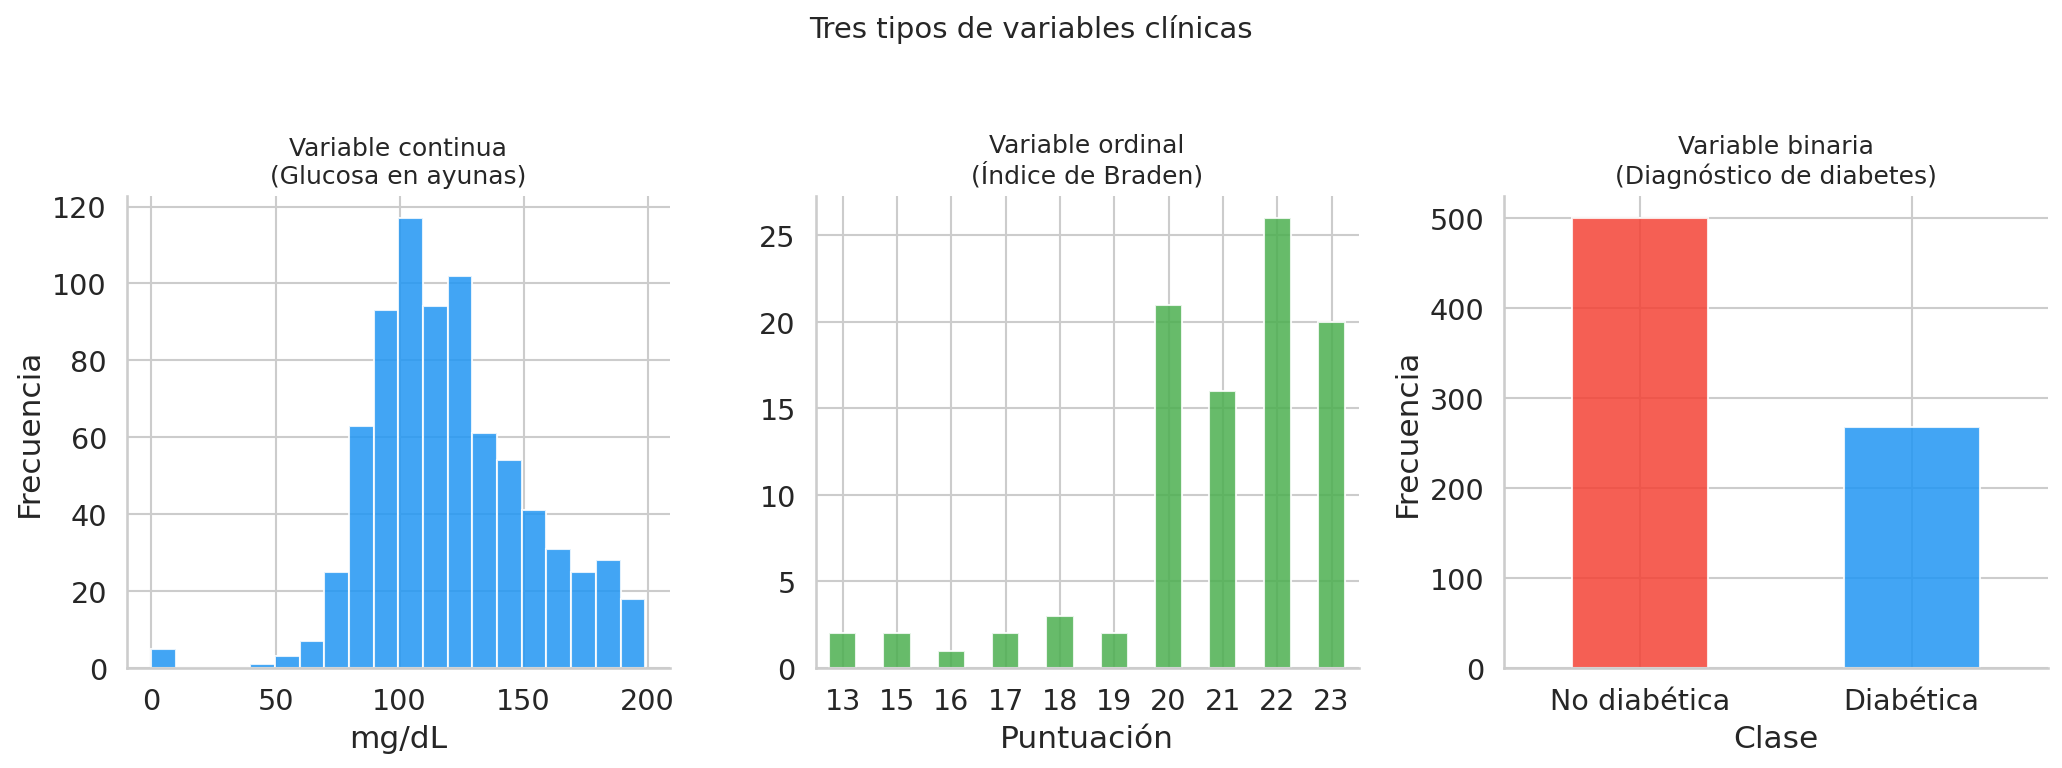
\includegraphics[width=\textwidth]{plots/16_tipos_variables_clinicas.png}
      \end{figure}
    \end{column}
  \end{columns}
\end{frame}

% SLIDE 7 - Valores cero imposibles ----------------------------------------
\begin{frame}{El problema de los ceros imposibles}
  \begin{columns}[T]
    \begin{column}{0.52\textwidth}
      \begin{block}{Diabetes Pima --- ceros biológicamente imposibles}
        \centering\vspace{2mm}
        \small
        \renewcommand{\arraystretch}{1.3}
        \begin{tabular}{lcc}
          \toprule
          \textbf{Variable} & \textbf{Mín} & \textbf{Ceros} \\
          \midrule
          Glucosa (mg/dL)              & 0 & 5 \\
          Presión diastólica (mmHg)    & 0 & 35 \\
          Pliegue tricipital (mm)      & 0 & 227 \\
          Insulina (uU/mL)             & 0 & 374 \\
          IMC (kg/m$^2$)               & 0 & 11 \\
          \bottomrule
        \end{tabular}
        \vspace{2mm}
      \end{block}
    \end{column}
    \begin{column}{0.45\textwidth}
      \begin{block}{A primera vista}
        \begin{figure}[H]
          \centering
          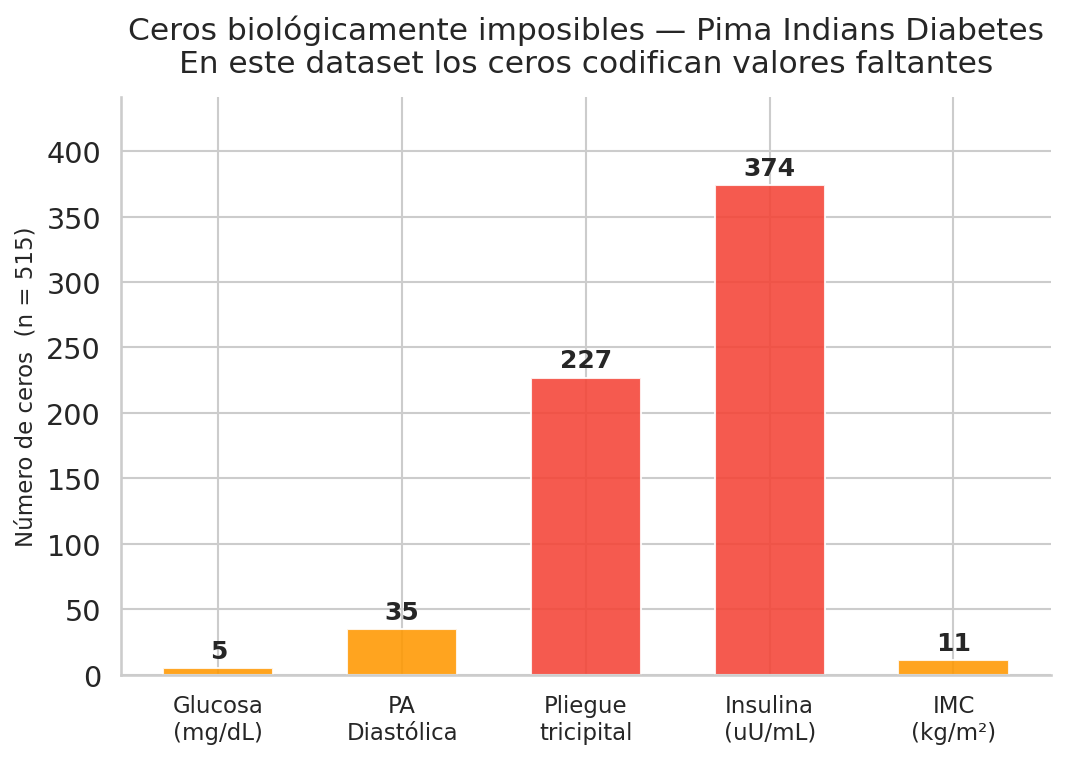
\includegraphics[width=\textwidth]{plots/19_diabetes_ceros_barras.png}
        \end{figure}
      \end{block}
    \end{column}
  \end{columns}
\end{frame}

% SLIDE 8 - Outliers -------------------------------------------------------
\begin{frame}{Outliers --- ¿Error o hallazgo real?}
  \begin{columns}[T]
    \begin{column}{0.52\textwidth}
      \begin{block}{Enzimas hepáticas --- Liver Disorders (n\,=\,232)}
        \begin{figure}[H]
          \centering
          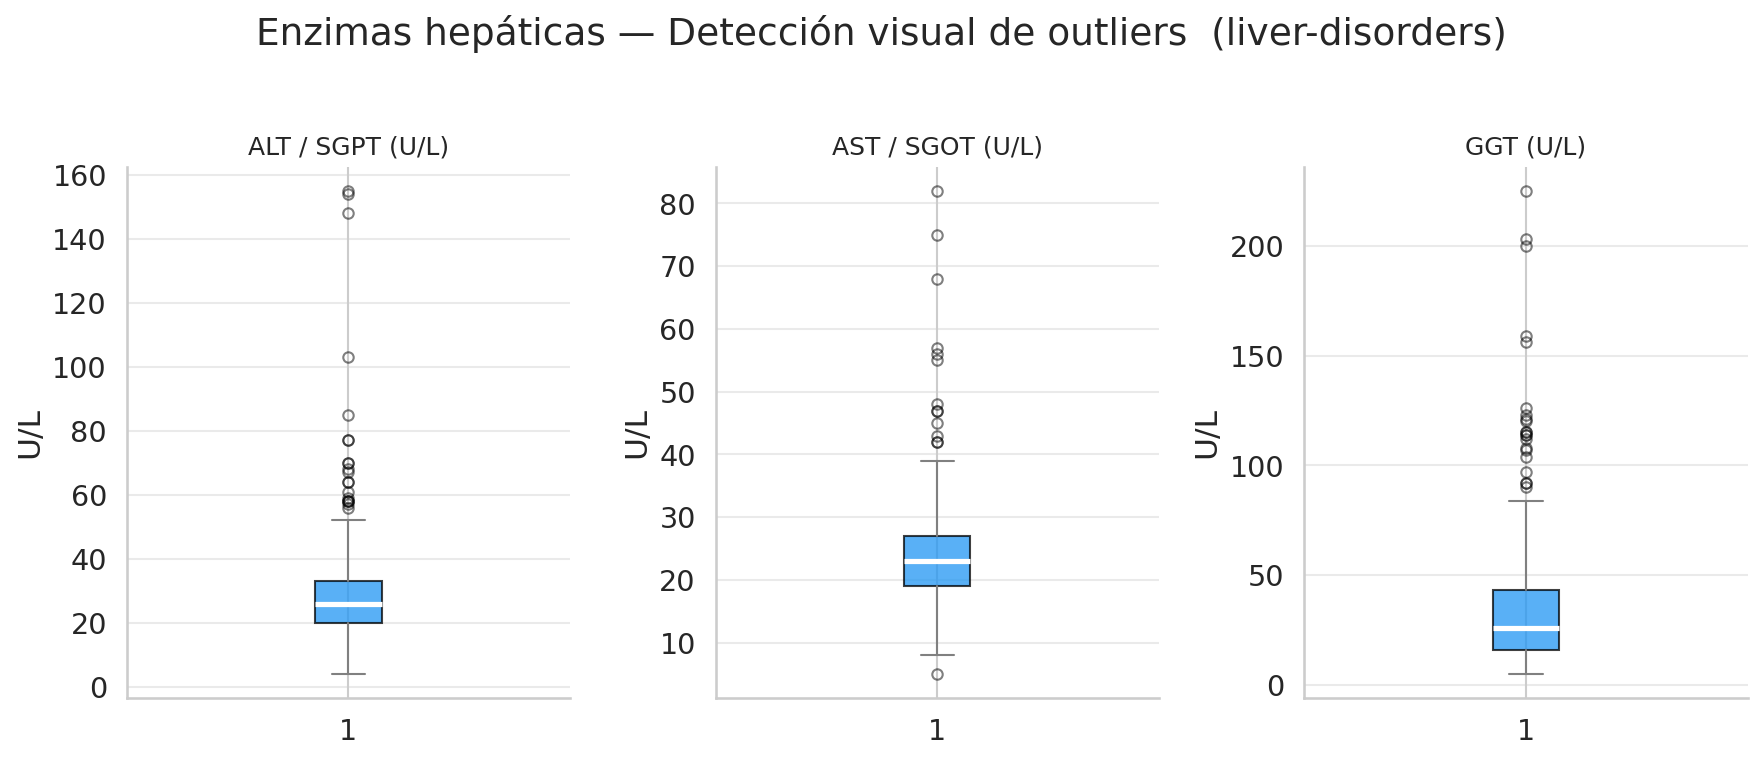
\includegraphics[width=\textwidth]{plots/10_liver_enzimas_boxplot.png}
        \end{figure}
        {\scriptsize SGPT\,=\,155 U/L\quad\textbf{¿Lo elimino?}}
      \end{block}
    \end{column}
    \begin{column}{0.45\textwidth}
      \vspace{4mm}
      \begin{block}{Regla de oro} \small
        \textbf{NO} sin investigar.\\[0.5mm]
        Un outlier no se borra: \textbf{se investiga.}
      \end{block}
      \vspace{0.5mm}
      \begin{itemize}\small
        \item Puede ser un error de entrada (decimal de más)
        \item Puede ser daño hepático agudo grave real
        \item Puede ser el caso más informativo del dataset
      \end{itemize}
      \vspace{2mm}
      \begin{block}{}
        \scriptsize El contexto clínico decide, no el algoritmo.\\[2mm]
        Siempre documentar la decisión en métodos.\\[1mm]
        Un BMI\,=\,67 es inusual pero biológicamente posible:\\
        obesidad mórbida grado III.
      \end{block}
    \end{column}
  \end{columns}
\end{frame}

% SLIDE 9 - Sesgos --------------------------------------------------------
\begin{frame}{Sesgos: cuando los datos nos engañan}
  {\small\color{UCgray} Tres trampas frecuentes que sesgan los resultados sin que nadie lo vea:}
  \vspace{3mm}
  \begin{columns}[T]
    \begin{column}{0.52\textwidth}
      \begin{block}{Sesgo de selección}
        \small Estudiáis toxicidad usando solo pacientes
        que \textbf{completaron} el tratamiento.\\[2mm]
        Excluisteis a los que lo abandonaron
        \textit{por la toxicidad}.\\
        \scriptsize Vuestra muestra ya no es representativa.
      \end{block}
      \vspace{3mm}
      \begin{block}{Sesgo de confusión}
        \small Hospitales con más médicos por cama\\
        $\rightarrow$ mayor mortalidad ($p<0{,}001$).\\[2mm]
        \textit{¿Los médicos matan pacientes?}\\[1mm]
        \scriptsize No. Los hospitales de \textbf{referencia regional}\\
        concentran los casos más graves \textit{y} tienen más personal.
      \end{block}
    \end{column}
    \begin{column}{0.45\textwidth}
      \begin{block}{Sesgo de información}
        \small Pacientes con más visitas acumulan
        más diagnóstico.\\[2mm]
        \scriptsize No porque estén más enfermos: porque tuvieron más oportunidades de ser diagnosticados.
      \end{block}
      \vspace{3mm}
      \begin{exampleblock}{La única defensa}
        \scriptsize Definir los criterios de inclusión/exclusión \textbf{antes} de abrir los datos.
      \end{exampleblock}
    \end{column}
  \end{columns}
\end{frame}

% SLIDE 10 - Mapa missings -------------------------------------------------
\begin{frame}{Valores faltantes --- El problema invisible}
  \begin{columns}[T]
    \begin{column}{0.52\textwidth}
      \begin{block}{Dataset Hipotiroidismo (n\,=\,3.163)}
        \begin{figure}[H]
          \centering
          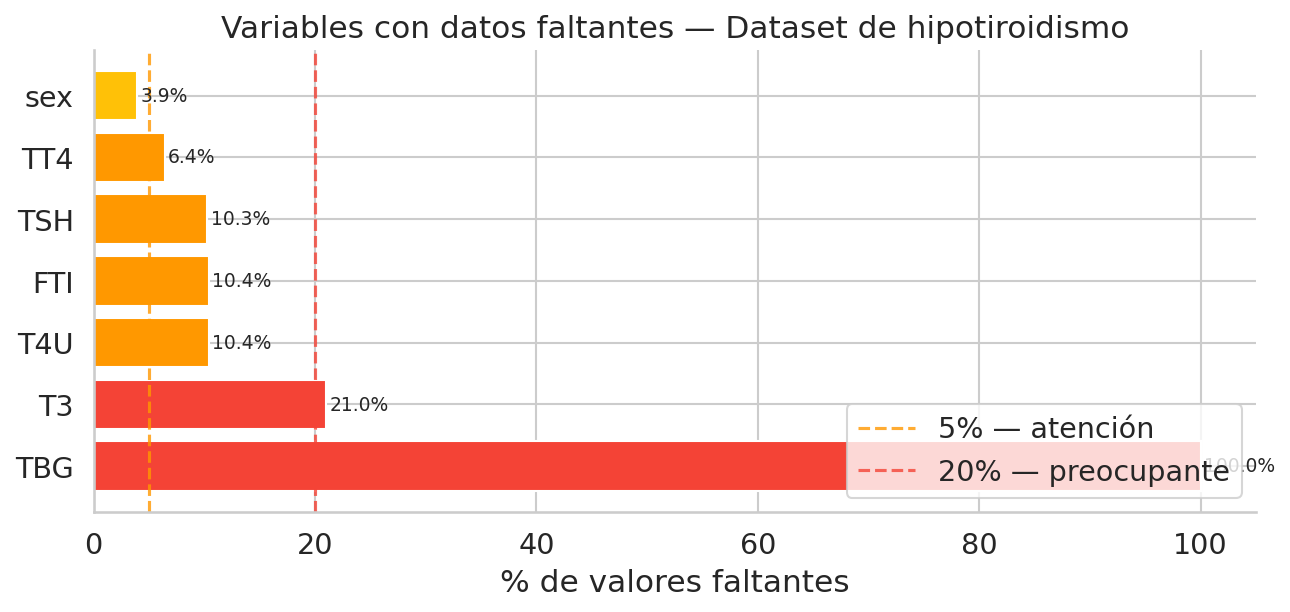
\includegraphics[width=\textwidth]{plots/08_hypothyroid_missing_values.png}
        \end{figure}
        {\scriptsize T3: 21\,\% faltantes\quad TSH: 10\,\%\quad TT4: 6\,\%}
      \end{block}
    \end{column}
    \begin{column}{0.45\textwidth}
      \vspace{4mm}
      \begin{block}{\large\centering ¿Por qué falta ese dato?}
        \vspace{2mm}
        \small La respuesta cambia por completo el análisis.
      \end{block}
      \vspace{0.5mm}
      \begin{itemize}\small
        \item No todos los missings son iguales
        \item Eliminar filas sin razonar introduce sesgo
        \item Falta más en un grupo $\rightarrow$ sesgo de selección
      \end{itemize}
      \vspace{4mm}
      \begin{block}{Umbrales prácticos}
        \scriptsize $<5$\,\% tolerable en la mayoría de casos\\
        $>20$\,\% en variable clave: declararlo en métodos\\
        $>40$\,\% en variable clave: replantearse si incluirla
      \end{block}
    \end{column}
  \end{columns}
\end{frame}

% SLIDE 11 - Tipos de missings ---------------------------------------------
\begin{frame}{Los tres tipos de datos faltantes}
  \begin{columns}[T]
    \begin{column}{0.64\textwidth}
      \centering\vspace{2mm}
      \begin{tikzpicture}[scale=0.80,transform shape,node distance=0.4cm]
        \tikzset{mcar/.style={rectangle,draw=UCblue,fill=UCbluePale,
                 minimum width=6.8cm,minimum height=1.55cm,
                 text centered,font=\small,rounded corners=0.15cm,
                 text width=6.5cm}}
        \tikzset{mar/.style={mcar,draw=UCgreen!70!black,fill=UCgreen!10}}
        \tikzset{mnar/.style={mcar,draw=UCred,fill=UCred!8}}
        \node[mcar] (b1) at (0,0) {%
          \textbf{MCAR --- Missing Completely At Random}\\[2pt]
          \small La enfermera olvidó anotar la temperatura.\\
          \textit{Falta totalmente al azar.}};
        \node[mar]  (b2) at (0,-2.3) {%
          \textbf{MAR --- Missing At Random}\\[2pt]
          \small No se midió la glucosa porque el paciente llegó en coma.\\
          \textit{Falta por razones observables en otras variables.}};
        \node[mnar] (b3) at (0,-4.6) {%
          \textbf{MNAR --- Missing Not At Random}\enspace{\color{UCred}\bfseries\scriptsize$\leftarrow$ más peligroso}\\[2pt]
          \small El paciente no declaró que fumaba\ldots\\
          \textbf{precisamente porque fumaba.}\\
          \textit{Falta por el propio valor que falta.}};
        \draw[->,thick,UCblue!50]  (b1.south) -- (b2.north);
        \draw[->,thick,UCgreen!60] (b2.south) -- (b3.north);
      \end{tikzpicture}
    \end{column}
    \begin{column}{0.33\textwidth}
      \vspace{6mm}
      \begin{exampleblock}{Regla}
        \small \textbf{¿Por qué falta ese dato?}\\[2mm]
        \scriptsize Preguntad al clínico.
        Su respuesta determina el análisis.
      \end{exampleblock}
      \vspace{4mm}
      \begin{block}{MNAR: sesgo invisible}
        \scriptsize Al borrar esas filas el análisis \textit{parece} correcto.\\[2mm]
        \textbf{No lo es.}
      \end{block}
    \end{column}
  \end{columns}
\end{frame}

% SLIDE 12 - Lista de verificación antes de analizar ----------------------
\begin{frame}{Antes de analizar: cinco preguntas obligatorias}
  \begin{columns}[T]
    \begin{column}{0.52\textwidth}
      \centering\vspace{4mm}
      \begin{tikzpicture}[scale=0.78,transform shape]
    \tikzset{
        caja/.style={
            rectangle,
            draw=UCblue,
            fill=UCbluePale,
            minimum width=6.8cm,
            minimum height=0.72cm,
            text centered,
            font=\small,
            rounded corners=0.12cm,
            text width=6.5cm
        }
    }

    \node[caja] (p1) at (0,0)     {\textbf{1.} ¿Está definida la variable de desenlace?};
    \node[caja] (p2) at (0,-1.6)  {\textbf{2.} ¿Sabéis qué significa cada columna?};
    \node[caja] (p3) at (0,-3.2)  {\textbf{3.} ¿Habéis revisado mínimos y máximos?};
    \node[caja] (p4) at (0,-4.8)  {\textbf{4.} ¿Sabéis por qué faltan esos datos?};
    \node[caja,draw=UCgreen,fill=UCgreen!12] (p5) at (0,-6.4)
        {\textbf{5.} ¿Hay outliers que investigar?};

    \draw[->,thick,UCblue!60] (p1.south) -- (p2.north);
    \draw[->,thick,UCblue!60] (p2.south) -- (p3.north);
    \draw[->,thick,UCblue!60] (p3.south) -- (p4.north);
    \draw[->,thick,UCblue!60] (p4.south) -- (p5.north);
\end{tikzpicture}
    \end{column}
    \begin{column}{0.45\textwidth}
        \vspace{4mm}
        \begin{block}{El peligro real}
        \small Un análisis sobre datos sucios produce resultados incorrectos \textbf{que parecen correctos.}\\[3mm]
        \scriptsize El peligro no es que el programa falle.\\
        El peligro es que el programa funcione.
      \end{block}    
      \vspace{3mm}
      \begin{block}{La pregunta más importante}
        \small ¿Qué queréis saber \textbf{exactamente}?\\[2mm]
        \scriptsize Definidla antes de abrir cualquier archivo.\\
        Una pregunta mal formulada produce\\
        respuestas irrelevantes, aunque sean correctas.
      \end{block}
    \end{column}
  \end{columns}
  \note{Este slide es el puente entre calidad de datos y estadística. El peligro no es el error --- es el error silencioso.}
\end{frame}

% SLIDE 13 - Que es modelizacion descriptiva --------------------------------
\begin{frame}{Modelización descriptiva: qué es (y qué no es)}
  \begin{columns}[T]
    \begin{column}{0.50\textwidth}
      \begin{block}{LO QUE NO ES}
        \begin{itemize}\small
          \item \no\ Ajustar una regresión logística
          \item \no\ Construir un clasificador de ML
          \item \no\ Predecir lo que le pasará al próximo paciente
        \end{itemize}
      \end{block}
      \vspace{3mm}
      \begin{exampleblock}{LO QUE SÍ ES}
        \begin{itemize}\small
          \item \yes\ Caracterizar quiénes son los pacientes
          \item \yes\ Describir cómo se distribuyen las variables
          \item \yes\ Identificar patrones y relaciones
          \item \yes\ Detectar anomalías, missings y sesgos
          \item \yes\ Generar hipótesis para análisis futuros
        \end{itemize}
      \end{exampleblock}
    \end{column}
    \begin{column}{0.47\textwidth}
      \vspace{3mm}
      \begin{block}{Los cuatro niveles}
        \centering\vspace{2mm}
        \begin{tikzpicture}[scale=0.80,transform shape]
          \tikzset{s/.style={rectangle,draw=UCblue,fill=UCbluePale,
                   minimum width=4.8cm,minimum height=0.60cm,
                   text centered,font=\scriptsize,rounded corners=0.1cm}}
          \tikzset{sg/.style={s,fill=UCgray!12,draw=UCgray!40,text=UCgray}}
          \node[s]  (d) at (0, 0)   {Descriptivo: \textit{¿Cómo son mis datos?}};
          \node[s]  (i) at (0,-0.9) {Inferencial: \textit{¿Hay diferencia real?}};
          \node[sg] (p) at (0,-1.8) {Predictivo: \textit{¿Qué pasará al siguiente?}};
          \node[sg] (r) at (0,-2.7) {Prescriptivo: \textit{¿Qué debo hacer?}};
          \draw[->,thick,UCblue!70]       (d.south) -- (i.north);
          \draw[->,thick,UCgray!50,dashed](i.south) -- (p.north);
          \draw[->,thick,UCgray!50,dashed](p.south) -- (r.north);
        \end{tikzpicture}
        \vspace{2mm}\\
        {\scriptsize El descriptivo bien hecho es la\\
        \textbf{base obligatoria} de cualquier análisis riguroso.}
      \end{block}
    \end{column}
  \end{columns}
\end{frame}

% SLIDE 14 - Mensaje clave bloque 1 ----------------------------------------
\begin{frame}
  \begin{center}
    \vspace{4mm}
    {\color{UCblue!30}\rule{\textwidth}{1.5pt}}
    \vspace{6mm}
    \begin{beamercolorbox}[sep=18pt,center,rounded=true,shadow=true]{block title}
      \LARGE\bfseries Conoce tus datos antes de analizarlos.
    \end{beamercolorbox}
    \vspace{6mm}
    {\Large Un buen análisis de calidad de datos tarda poco.}\\[4mm]
    {\Large Evita meses de revisiones.}
    \vspace{6mm}
    {\color{UCblue!30}\rule{\textwidth}{1.5pt}}
  \end{center}
\end{frame}


% =========================================================================
\section{Estadística descriptiva}
% =========================================================================

% Separador bloque 2 -------------------------------------------------------
\begin{frame}[plain]
  \begin{center}
    \vspace{14mm}
    \begin{beamercolorbox}[sep=22pt,center,rounded=true,shadow=true]{block title}
      {\large Bloque 2}\\[4mm]
      \LARGE\bfseries Estadística descriptiva
    \end{beamercolorbox}
    \vspace{8mm}
    {\large\color{UCgray} Table~1, distribuciones y tests.}
  \end{center}
\end{frame}

% SLIDE 16 - El Table 1 ---------------------------------------------------
\begin{frame}{El Table~1 --- La tabla más leída de cualquier artículo}
  \begin{columns}[T]
    \begin{column}{0.50\textwidth}
      \begin{itemize}\small
        \item Todo lector va \textbf{primero} al Table~1.
        \item Responde: \textit{¿a quién le hicieron esto?}
        \item Sin él, los resultados son números sin contexto.
        \item \textbf{Muchos revisores lo leen y ya saben si el estudio es serio.}
      \end{itemize}
      \vspace{3mm}
      \begin{block}{Anatomía del Table~1}
        \begin{itemize}\scriptsize
          \item Continuas: Media\,$\pm$\,SD \quad o \quad Mediana [IQR]
          \item Categóricas: $n$ (\%)
          \item $p$-valor entre grupos (con cautela)
          \item ¿Media o mediana? La distribución lo dice en 5 s.
        \end{itemize}
      \end{block}
    \end{column}
    \begin{column}{0.47\textwidth}
      \begin{exampleblock}{Table~1 real --- Diabetes Pima (n\,=\,515)}
        \centering\scriptsize
        \renewcommand{\arraystretch}{1.3}
        \begin{tabular}{lcc}
          \toprule
          \textbf{Variable} & \textbf{Sin DM} & \textbf{Con DM} \\
                            & (n\,=\,339) & (n\,=\,176) \\
          \midrule
          Glucosa (mg/dL)   & $110\pm24$       & $142\pm30$ \\
          IMC (kg/m$^2$)    & $31\pm7$         & $35\pm7$ \\
          Edad (años)       & 27 [23--37]      & 36 [28--45] \\
          Insulina (uU/mL)  & 100 [66--156]    & 176 [130--238] \\
          Embarazos         & 2 [1--5]         & 5 [2--8] \\
          \midrule
          \multicolumn{3}{l}{\scriptsize $p<0{,}001$ en todas las variables}\\
          \bottomrule
        \end{tabular}
      \end{exampleblock}
    \end{column}
  \end{columns}
  \note{El Table 1 bien elaborado ya desvela los marcadores más relevantes, sin ejecutar ningún modelo.}
\end{frame}

% SLIDE 17 - Media vs mediana ---------------------------------------------
\begin{frame}{Media vs.\ mediana --- La distribución manda}
  \begin{columns}[T]
    \begin{column}{0.56\textwidth}
      \begin{block}{Glucosa plasmática --- Diabetes Pima}
        \begin{figure}[H]
          \centering
          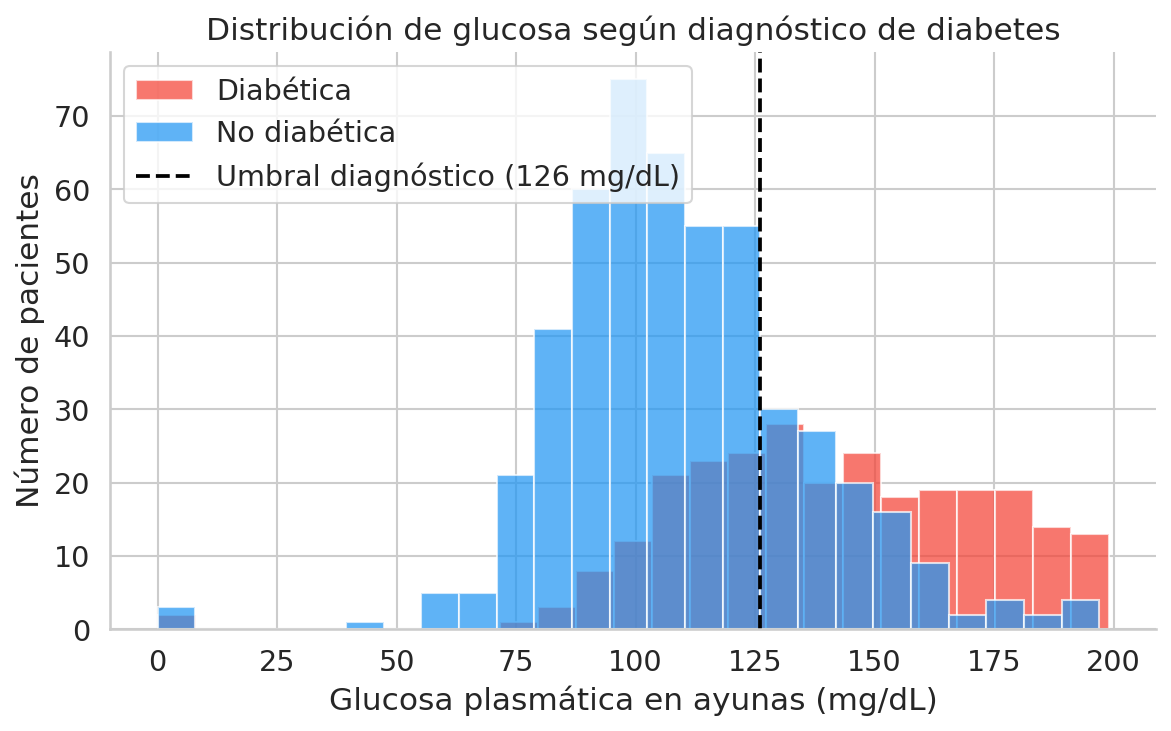
\includegraphics[width=\textwidth]{plots/01_diabetes_glucosa_histograma.png}
        \end{figure}
        {\scriptsize Umbral 126\,mg/dL: criterio ADA (1997)}
      \end{block}
    \end{column}
    \begin{column}{0.41\textwidth}
      \vspace{4mm}
      \begin{block}{Regla}
        \begin{itemize}\small
          \item \textbf{Simétrica} $\rightarrow$ Media\,$\pm$\,SD \yes
          \item \textbf{Sesgada} u outliers $\rightarrow$ Mediana [IQR] \yes
          \item \textbf{Bimodal} $\rightarrow$ dos poblaciones distintas
        \end{itemize}
      \end{block}
      \vspace{0.5mm}
      \begin{exampleblock}{}
        \scriptsize Insulina en Pima (sin missings, n\,=\,259):\\
        Media\,=\,156 vs.\ Mediana\,=\,120\,uU/mL.\\[1mm]
        Un outlier de 846 arrastra la media.\\
        Informar la media: historia equivocada.
      \end{exampleblock}
    \end{column}
  \end{columns}
\end{frame}

% SLIDE 18 - IMC boxplot --------------------------------------------------
\begin{frame}{IMC --- Cuando la distribución importa}
  \begin{columns}[T]
    \begin{column}{0.56\textwidth}
      \begin{block}{IMC según diabetes --- Pima Indians}
        \begin{figure}[H]
          \centering
          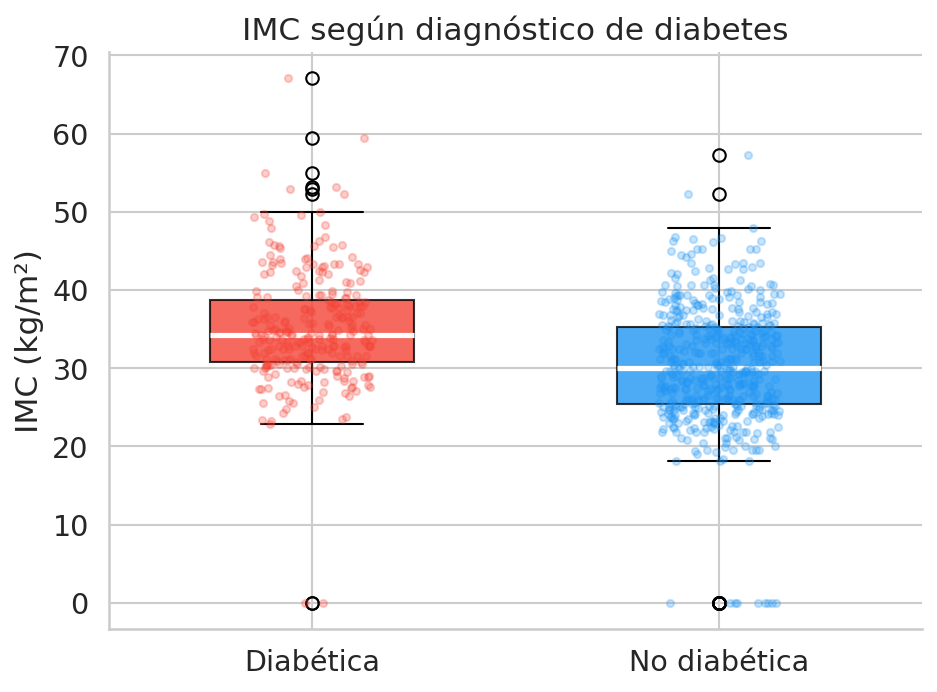
\includegraphics[width=\textwidth]{plots/02_diabetes_imc_boxplot.png}
        \end{figure}
      \end{block}
    \end{column}
    \begin{column}{0.41\textwidth}
      \vspace{4mm}
      \begin{block}{Lo que el boxplot revela}
        \begin{itemize}\small
          \item Mediana IMC-DM $>$ Mediana IMC-no-DM
          \item Distribución sesgada a la derecha en ambos
          \item Outliers en ambos grupos
          \item Solapamiento considerable
        \end{itemize}
      \end{block}
      \vspace{0.5mm}
      \begin{exampleblock}{}
        \small Diferencia clara pero no perfecta.\\
        Exactamente lo que vais a encontrar en vuestros datos reales.\\[2mm]
        \scriptsize Los datasets perfectamente separados son una rareza, no norma.
      \end{exampleblock}
    \end{column}
  \end{columns}
\end{frame}

% SLIDE 19 - La regla unificada -------------------------------------------
\begin{frame}{Una sola regla --- Tres aplicaciones}

\begin{block}{Regla práctica}
\centering
\small
¿Forma de campana? $\rightarrow$ \textbf{estadísticos clásicos} \hspace{1cm}
¿Cola larga? $\rightarrow$ \textbf{estadísticos robustos}
\end{block}

\vspace{2mm}

\small
\renewcommand{\arraystretch}{1.3}
\begin{tabular}{p{3.0cm} p{3.2cm} p{3.2cm}}
\toprule
\textbf{Tarea} & \textbf{Campana} & \textbf{Cola larga} \\
\midrule
Describir & Media $\pm$ SD & Mediana [IQR] \\
Comparar & $t$ de Student & Mann--Whitney U \\
Asociación & Pearson ($r$) & Spearman ($\rho$) \\
\bottomrule
\end{tabular}

\vspace{3mm}

\begin{columns}[T,onlytextwidth]
\column{0.48\textwidth}
\begin{exampleblock}{Ejemplos}
\footnotesize
Glucosa e IMC\\
$\rightarrow$ Media, $t$, Pearson
\end{exampleblock}

\column{0.48\textwidth}
\begin{block}{Ejemplos}
\footnotesize
Insulina y Edad\\
$\rightarrow$ Mediana, Mann--Whitney, Spearman
\end{block}
\end{columns}

\note{Esta tabla es el corazón de la sesión y resume la regla que se repetirá posteriormente.}

\end{frame}

% SLIDE 20 - El p-valor ---------------------------------------------------
\begin{frame}{El $p$-valor: qué es y qué \textbf{no} es}
  \begin{columns}[T]
    \begin{column}{0.48\textwidth}
      \vspace{2mm}
      \begin{block}{¿Qué significa $p < 0{,}05$?}
        \small ``Si los dos grupos fueran \textbf{iguales} de verdad,\\
        la probabilidad de ver esta diferencia\\
        \textbf{solo por azar} sería menor del 5\,\%.''\\[2mm]
        \scriptsize Es decir: la diferencia probablemente no es ruido.\\
        No dice nada más.
      \end{block}
      \vspace{4mm}
      \begin{block}{Lo que \textbf{no} significa}
        \begin{itemize}\small
          \item \no\ La diferencia es grande o importante
          \item \no\ Hay que cambiar la práctica clínica
          \item \no\ Una cosa \textit{causa} la otra
        \end{itemize}
      \end{block}
    \end{column}
    \begin{column}{0.48\textwidth}
      \vspace{2mm}
      \begin{exampleblock}{El problema con muestras grandes}
        \small Con \textbf{10.000 pacientes}, una diferencia\\
        de \textbf{0{,}1 mmHg} en presión arterial\\
        puede dar $p < 0{,}001$.\\[2mm]
        \scriptsize Estadísticamente significativo.\\
        Clínicamente irrelevante.
      \end{exampleblock}
      \vspace{4mm}
      \begin{block}{La pregunta correcta}
        \small ¿Cuánto es la diferencia?\\
        ¿Esa diferencia importa para el paciente?\\[1mm]
        \scriptsize El $p$-valor no responde ninguna de las dos.
      \end{block}
    \end{column}
  \end{columns}
\end{frame}

% SLIDE 21 - Correlación no implica causalidad --------------------------------
\begin{frame}{Correlación $\neq$ causalidad}
  \begin{center}
    {
\setbeamercolor{block title alerted}{fg=black}
\begin{beamercolorbox}[sep=8pt,center,rounded=true,shadow=false]{block title alerted}
\normalsize\bfseries
Una correlación estadística no prueba que una cosa \textit{cause} la otra.
\end{beamercolorbox}
}
  \end{center}
  \begin{columns}[T]
    \begin{column}{0.48\textwidth}
      \begin{block}{Ejemplo clínico}
        \small Hospitales con más médicos por cama\\
        $\rightarrow$ mayor mortalidad.\\[2mm]
        \textit{¿Los médicos matan pacientes?}\\[2mm]
        \scriptsize No. Los hospitales principales tratan\\
        los casos más graves. La complejidad del caso\\
        es la variable que explica ambas cosas.
      \end{block}
    \end{column}
    \begin{column}{0.48\textwidth}
      \begin{block}{Ejemplo clásico}
        \small Países con mayor consumo de chocolate\\
        tienen más premios Nobel per cápita.\\[2mm]
        \scriptsize La correlación es real.\\
        La causalidad, absurda.\\[1mm]
        Ambas variables correlacionan con\\
        la riqueza del país.
      \end{block}
    \end{column}
  \end{columns}
  \vspace{4mm}
  \begin{exampleblock}{\centering}
    \centering\small
    Antes de concluir causalidad: \textbf{¿hay una tercera variable que explique ambas?}
  \end{exampleblock}
\end{frame}

% SLIDE 22 - Correlaciones heatmap ----------------------------------------
\begin{frame}{Correlaciones --- Panorámica de relaciones}
  \begin{columns}[T]
    \begin{column}{0.52\textwidth}
      \begin{block}{Heatmap --- Diabetes Pima}
        \begin{figure}[H]
          \centering
          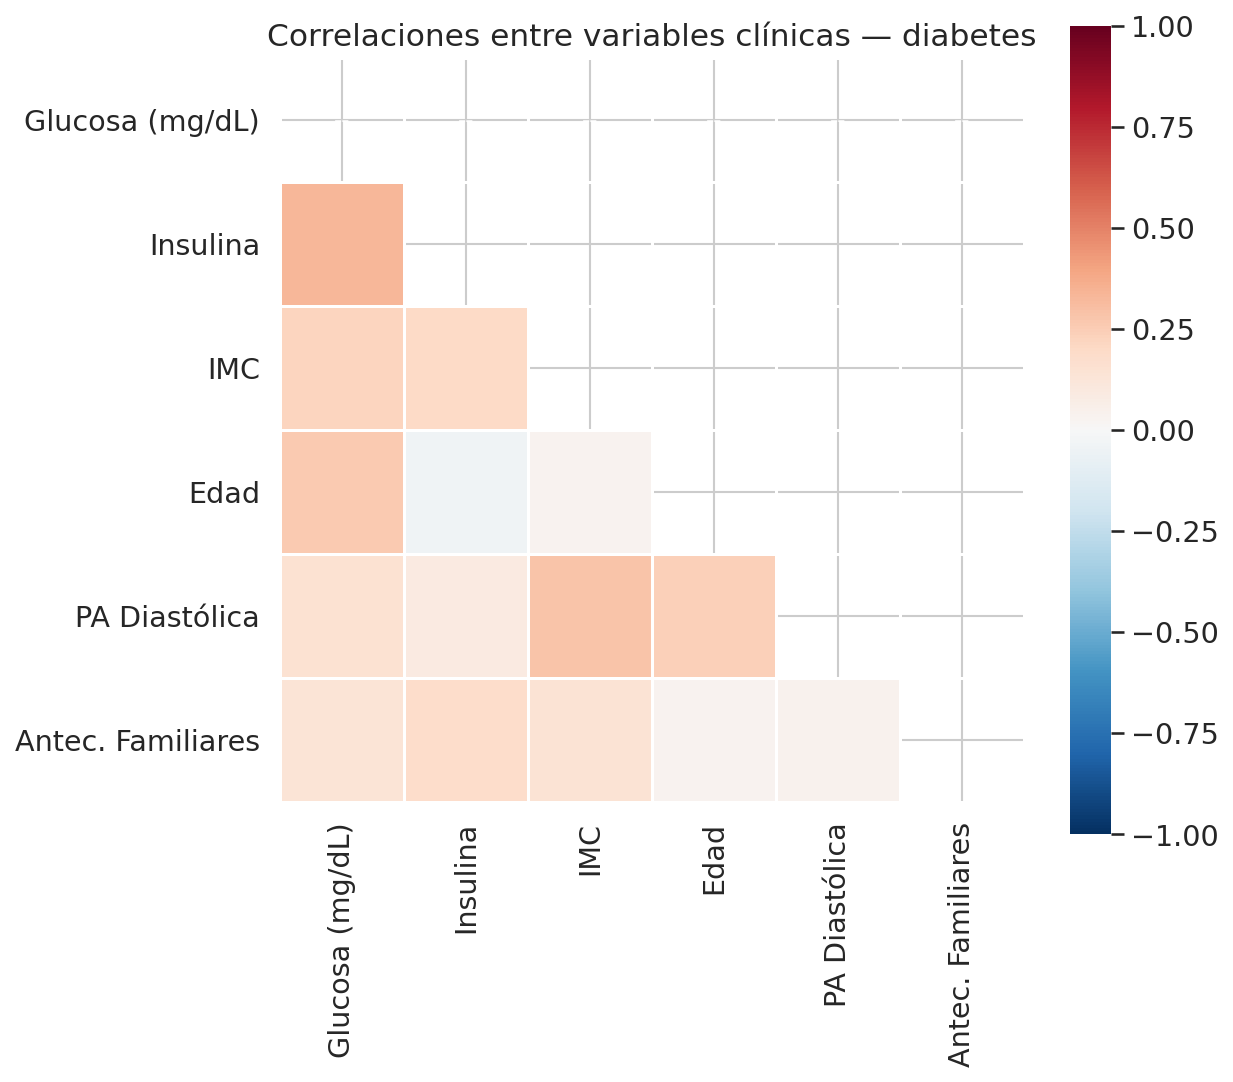
\includegraphics[width=\textwidth]{plots/03_diabetes_correlaciones_heatmap.png}
        \end{figure}
      \end{block}
    \end{column}
    \begin{column}{0.45\textwidth}
      \vspace{4mm}
      \begin{itemize}\small
        \item Glucosa e insulina: correlacionadas (esperado)
        \item IMC y pliegue cutáneo: correlacionadas (lógico)
      \end{itemize}
      \vspace{4mm}
      \begin{block}{Multicolinealidad}
        \small Dos variables muy correlacionadas\\
        \textbf{no deben entrar juntas en un modelo.}\\[2mm]
        \scriptsize Los coeficientes se inflan o invierten.\\
        El modelo es matemáticamente correcto\\
        pero clínicamente ininterpretable.
      \end{block}
    \end{column}
  \end{columns}
\end{frame}

% SLIDE 23 - Table 1 tumor neuroendocrino (Metastasis) -----------------------
\begin{frame}{Table~1 con datos reales --- Tumor neuroendocrino (Metastasis, n\,=\,493)}
  \begin{columns}[T]
    \begin{column}{0.54\textwidth}
      \begin{block}{Factores asociados a metástasis --- Sin vs.\ Con}
  \centering
  \scriptsize
  \renewcommand{\arraystretch}{1.15}

  \resizebox{\linewidth}{!}{%
  \begin{tabular}{lccc}
    \toprule
    \textbf{Variable} & \textbf{Sin met.} & \textbf{Con met.} & $p$ \\
                      & (n\,=\,327)       & (n\,=\,166)       & \\
    \midrule
    Edad (años)        & 44 [30--58]      & 38 [25--50]       & 0{,}001\\
    NMN (pg/mL)        & 592 [232--1563]  & 985 [219--2678]   & 0{,}026\\
    MN (pg/mL)         & 114 [37--492]    & 34 [21--59]       & $<0{,}001$\\
    Volumen tumor (mL) & 20 [7--56]       & 96 [35--231]      & $<0{,}001$\\
    Extra-adrenal (\%) & 17\,\%           & 71\,\%            & $<0{,}001$\\
    SDHB+ (\%)         & 5\,\%            & 45\,\%            & $<0{,}001$\\
    \bottomrule
  \end{tabular}%
  }

  \vspace{1mm}
  {\scriptsize Mediana [IQR] para continuas; \% para categóricas}
\end{block}
    \end{column}
    \begin{column}{0.43\textwidth}
      \vspace{4mm}
      \begin{itemize}\small
        \item Volumen tumoral 5$\times$ mayor en metastásicos
        \item Localización extra-adrenal: de 17\,\% a 71\,\%
        \item SDHB+: de 5\,\% a 45\,\% --- marcador genético clave
        \item MN más baja en metastásicos: perfil bioquímico distinto
      \end{itemize}
      \vspace{4mm}
    \end{column}
  \end{columns}
\end{frame}

% SLIDE 24 - Que test usar -------------------------------------------------
\begin{frame}{¿Qué test estadístico usar?}
  \begin{columns}[T]
    \begin{column}{0.55\textwidth}
      \begin{block}{Tabla de decisión (cubre el 95\,\% de casos)}
        \centering\small
        \renewcommand{\arraystretch}{1.4}
        \begin{tabular}{p{2.8cm}p{1.9cm}p{1.9cm}}
          \toprule
          \textbf{Variable} & \textbf{Normal} & \textbf{No normal} \\
          \midrule
          Continua, 2 grupos & $t$-test & Mann-Whitney \\
          Continua, $>$2 gr. & ANOVA & Kruskal-Wallis \\
          Continua, pareada  & $t$-test par. & Wilcoxon \\
          Categórica (tabla) & \multicolumn{2}{c}{Chi$^2$ / Fisher} \\
          \bottomrule
        \end{tabular}
      \end{block}
      \vspace{3mm}
      \begin{exampleblock}{¿Cuándo es normal?}
        \scriptsize Ver el histograma. Forma de campana $\approx$ normal.\\
        Con $n<50$: el histograma no es suficiente, añadir un test de normalidad.\\
        Con $n>200$: cualquier test rechazará por desviaciones triviales.
      \end{exampleblock}
    \end{column}
    \begin{column}{0.42\textwidth}
      \vspace{3mm}
      \begin{block}{Regla de oro}
        Si tenéis dudas:\\
        \textbf{usad mediana y test no paramétrico.}\\[2mm]
        \scriptsize Perdéis algo de potencia estadística,
        pero nunca estaréis equivocados.
      \end{block}
      \vspace{3mm}
      \begin{block}{Fisher vs.\ chi-cuadrado}
        \scriptsize Chi$^2$: todas las celdas con $\geq 5$ observaciones.\\
        Fisher: cuando alguna celda tiene $<5$.\\[1mm]
        La mayoría de software lo aplica automáticamente.
      \end{block}
      \vspace{3mm}
      \begin{block}{}
        \scriptsize El test da el $p$-valor.\\
        La magnitud clínica la da el \textbf{tamaño del efecto}.\\
        Reportad ambos.
      \end{block}
    \end{column}
  \end{columns}
\end{frame}

% SLIDE 25 - TSH distribucion ----------------------------------------------
\begin{frame}{Distribuciones con cola larga --- ejemplo clínico}
  \begin{columns}[T]
    \begin{column}{0.56\textwidth}
      \begin{block}{TSH (hormona tiroidea) --- n\,=\,3.163 pacientes}
        \begin{figure}[H]
          \centering
          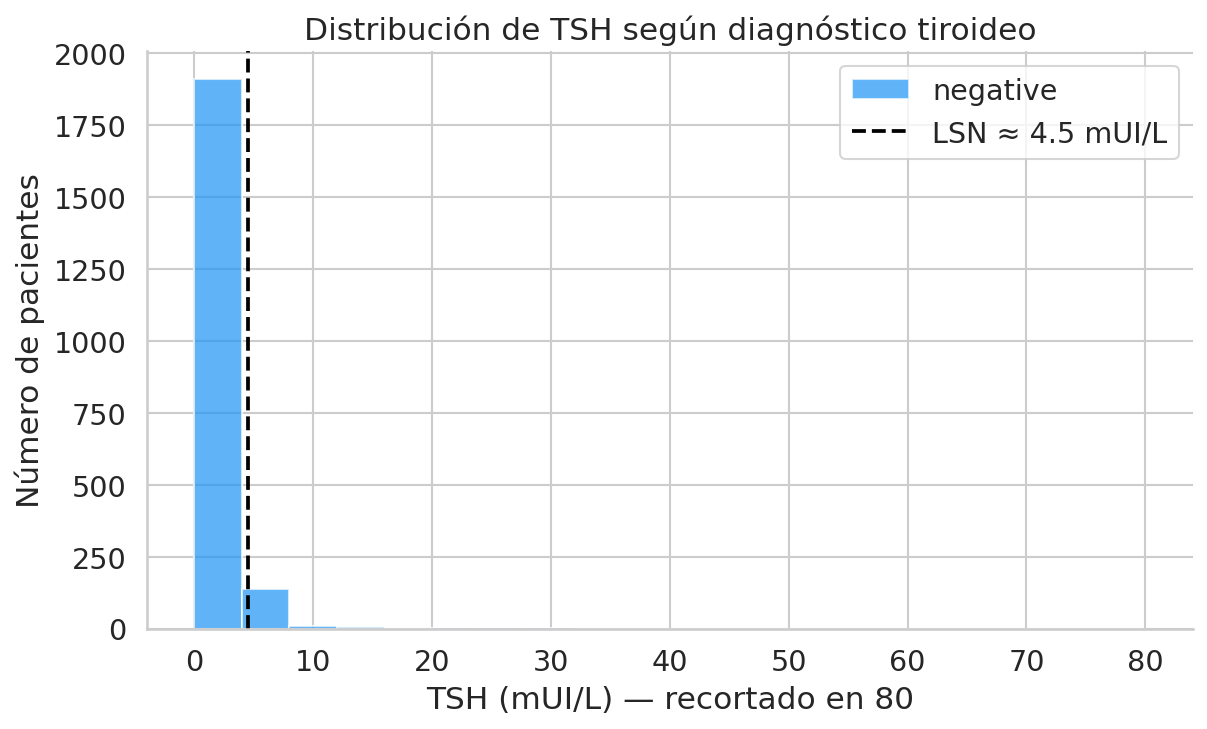
\includegraphics[width=\textwidth]{plots/09_hypothyroid_tsh_distribucion.png}
        \end{figure}
      \end{block}
    \end{column}
    \begin{column}{0.41\textwidth}
      \vspace{6mm}
      \begin{block}{Distribución sesgada a la derecha}
        \small Cola larga hacia valores altos.\\[2mm]
        Media $\gg$ Mediana.\\[2mm]
        Usando la media aquí\\
        \textbf{sobreestimáis} el valor típico.
      \end{block}
      \vspace{4mm}
      \begin{block}{}
        \scriptsize Otras variables con cola larga típica:\\[1mm]
        Estancia hospitalaria (días),\\
        ferritina, bilirrubina,\\
        troponina, enzimas hepáticas.\\[2mm]
        Analizar primero la forma,\\
        luego elegir el estadístico.
      \end{block}
    \end{column}
  \end{columns}
\end{frame}

% SLIDE 26 - Heatmap enzimas hepaticas ------------------------------------
\begin{frame}{Heatmap de enzimas hepáticas --- Liver Disorders}
  \begin{columns}[T]
    \begin{column}{0.50\textwidth}
      \begin{block}{Matriz de correlación --- n\,=\,232 pacientes}
        \begin{figure}[H]
          \centering
          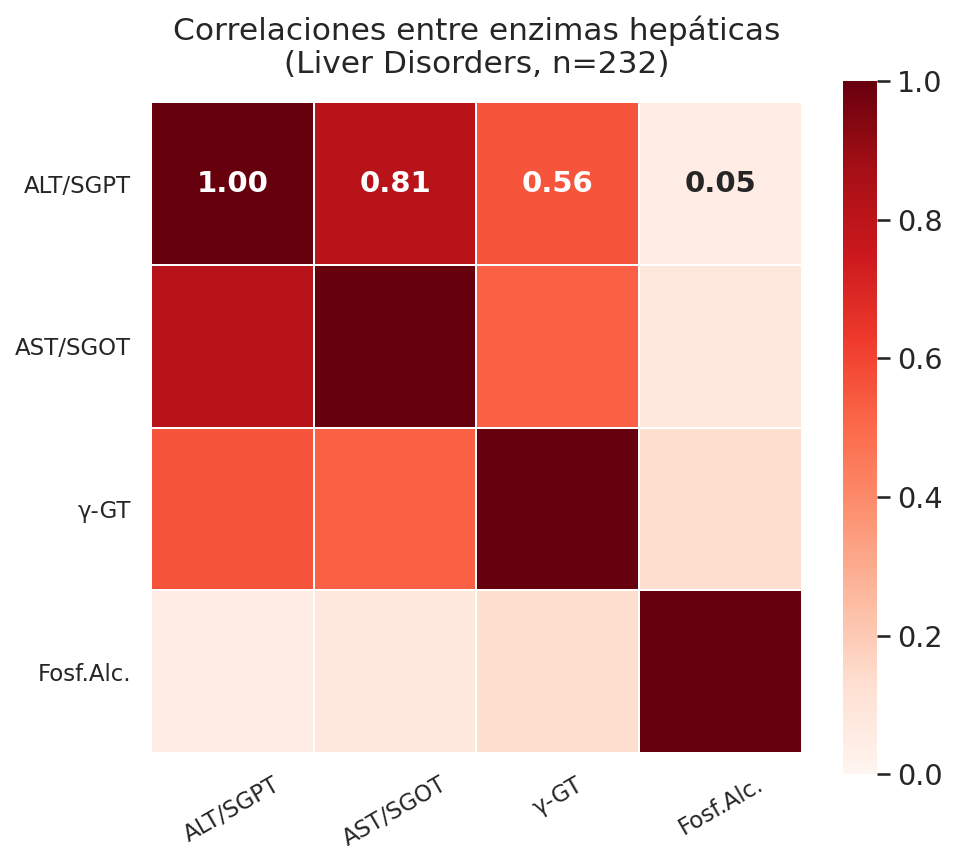
\includegraphics[width=\textwidth]{plots/17_liver_heatmap_correlaciones.png}
        \end{figure}
      \end{block}
    \end{column}
    \begin{column}{0.47\textwidth}
      \vspace{3mm}
      \begin{block}{Lo que revela la matriz}
        \begin{itemize}\small
          \item sgpt\,--\,sgot: $r=0{,}81$ --- alta correlación
          \item $\gamma$-GT\,--\,sgot: $r=0{,}53$ --- moderada
          \item alkphos: $r<0{,}15$ con todas las demás
        \end{itemize}
      \end{block}
      \vspace{3mm}
      \begin{block}{La biología detrás del número}
        \small sgpt y sgot suben juntas\\
        porque ambas marcan \textbf{daño hepatocelular}.\\[2mm]
        \scriptsize alkphos marca \textbf{colestasis}:
        un mecanismo completamente distinto.\\[2mm]
        El heatmap no muestra solo correlaciones.\\
        \textbf{Muestra la fisiopatología.}
      \end{block}
    \end{column}
  \end{columns}
  \note{Llevar siempre al clínico: el 0.81 tiene un nombre biológico. Eso es lo que hace útil la estadística descriptiva.}
\end{frame}

% SLIDE 27 - Scatter Gamma-GT vs drinks -----------------------------------
\begin{frame}{Cuando la correlación existe pero no la veis}
  \begin{columns}[T]
    \begin{column}{0.52\textwidth}
      \begin{block}{$\gamma$-GT vs.\ consumo de alcohol (n\,=\,232)}
        \begin{figure}[H]
          \centering
          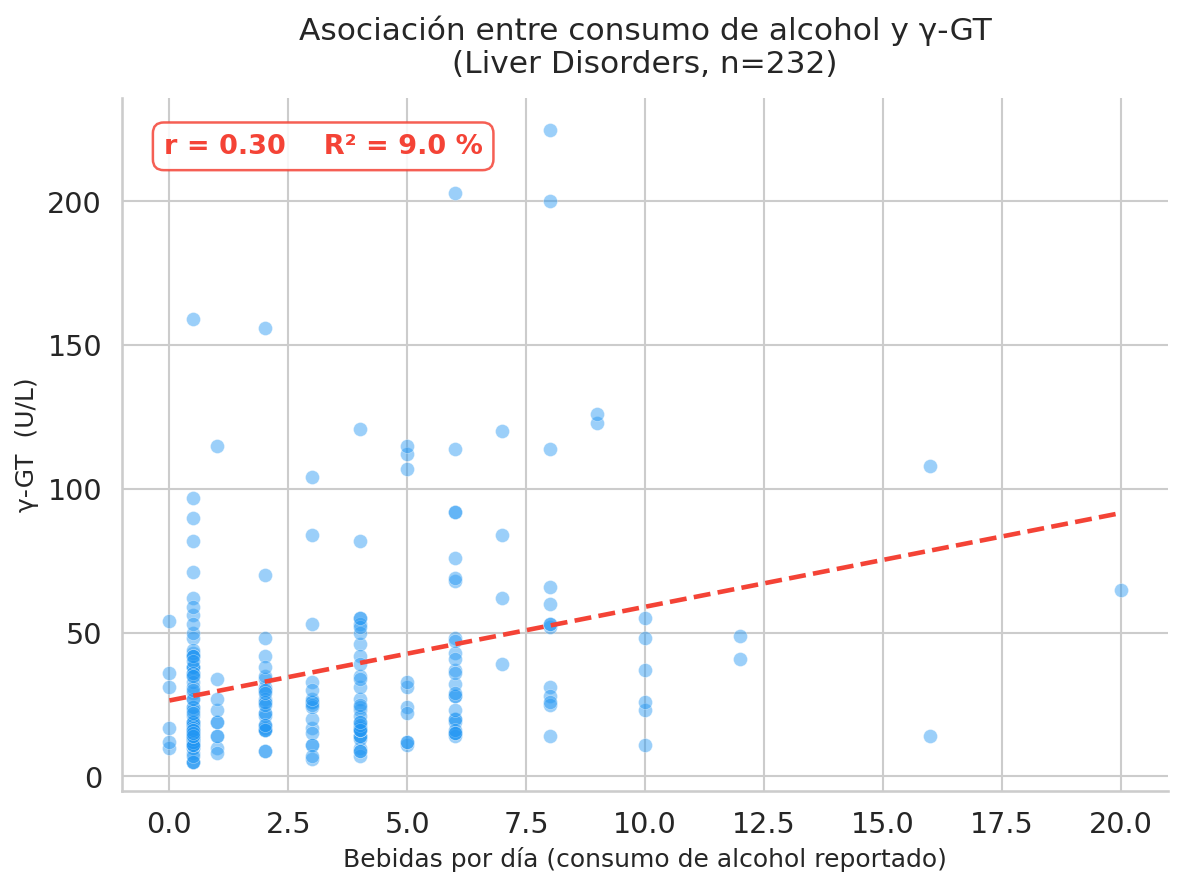
\includegraphics[width=\textwidth]{plots/18_liver_scatter_gammagt.png}
        \end{figure}
      \end{block}
    \end{column}
    \begin{column}{0.45\textwidth}
      \vspace{2mm}
      \begin{block}{Lo que muestra el gráfico}
        \begin{itemize}\small
          \item La nube de puntos es casi aleatoria
          \item La tendencia apenas se percibe
          \item $R^2 = 9$\,\%: el consumo explica\\
                solo 1 de cada 11 unidades de variabilidad
        \end{itemize}
      \end{block}
      \vspace{3mm}
      \begin{block}{Significativo $\neq$ relevante}
        \small Con $n=232$, $r=0{,}30$ da $p<0{,}001$.\\[2mm]
        El test detecta la asociación.\\
        \textbf{El gráfico muestra que es débil.}\\[2mm]
        \scriptsize Un resultado significativo con $R^2$ pequeño
        no cambia la práctica clínica.\\[1mm]
        \textbf{Reportad siempre el tamaño del efecto.}
      \end{block}
    \end{column}
  \end{columns}
  \note{Caso de uso fundamental: poner en perspectiva los p-valores. El gráfico hace en 2 segundos lo que el p-valor no puede hacer.}
\end{frame}

% SLIDE 28 - Mensaje clave bloque 2 ----------------------------------------
\begin{frame}
  \begin{center}
    \vspace{4mm}
    {\color{UCblue!30}\rule{\textwidth}{1.5pt}}
    \vspace{6mm}
    \begin{beamercolorbox}[sep=18pt,center,rounded=true,shadow=true]{block title}
      \LARGE\bfseries El Table~1 bien hecho ya es un resultado.
    \end{beamercolorbox}
    \vspace{6mm}
    {\Large No es relleno de la introducción.}\\[4mm]
    {\Large Es el primer resultado que le cuentas al lector.}
    \vspace{6mm}
    {\color{UCblue!30}\rule{\textwidth}{1.5pt}}
  \end{center}
\end{frame}

% =========================================================================
\section{Visualización}
% =========================================================================

% Separador bloque 3 -------------------------------------------------------
\begin{frame}[plain]
  \begin{center}
    \vspace{14mm}
    \begin{beamercolorbox}[sep=22pt,center,rounded=true,shadow=true]{block title}
      {\large Bloque 3}\\[4mm]
      \LARGE\bfseries Visualización
    \end{beamercolorbox}
    \vspace{8mm}
    {\large\color{UCgray} Las imágenes que convencen a los revisores.}
  \end{center}
\end{frame}

% SLIDE 30 - Caja de herramientas -----------------------------------------
\begin{frame}{La caja de herramientas visual}
  \begin{center}
    \begin{beamercolorbox}[sep=8pt,center,rounded=true]{block title example}
      \large Si no puedes explicar en \textbf{5 segundos} lo que muestra tu gráfico,
      el gráfico está mal hecho.
    \end{beamercolorbox}
  \end{center}
  \vspace{0.5mm}
  \begin{columns}[T]
    \begin{column}{0.24\textwidth}
      \begin{block}{\centering Histograma}
        \centering\scriptsize\vspace{1mm}
        \textbf{Una variable}\\[2mm]
        ¿Simétrica?\\¿Sesgada?\\¿Outliers?\\¿Bimodal?
        \vspace{1mm}
      \end{block}
    \end{column}
    \begin{column}{0.24\textwidth}
      \begin{block}{\centering Boxplot}
        \centering\scriptsize\vspace{1mm}
        \textbf{Comparar grupos}\\[2mm]
        Mediana, IQR,\\bigotes, outliers
        \vspace{1mm}
      \end{block}
    \end{column}
    \begin{column}{0.24\textwidth}
      \begin{block}{\centering Scatter plot}
        \centering\scriptsize\vspace{1mm}
        \textbf{Dos variables}\\[2mm]
        ¿Suben juntas?\\¿Grupos separados?
        \vspace{1mm}
      \end{block}
    \end{column}
    \begin{column}{0.24\textwidth}
      \begin{block}{\centering Heatmap}
        \centering\scriptsize\vspace{1mm}
        \textbf{Correlaciones}\\[2mm]
        Panorámica\\con $>5$ variables
        \vspace{1mm}
      \end{block}
    \end{column}
  \end{columns}
  \vspace{0.5mm}
  \begin{exampleblock}{\centering Regla de elección}
    \centering\scriptsize
    ¿Una variable? \textbf{Histograma.}\quad
    ¿Dos grupos? \textbf{Boxplot.}\quad
    ¿Dos variables continuas? \textbf{Scatter.}\quad
    ¿Muchas variables? \textbf{Heatmap.}
  \end{exampleblock}
\end{frame}

% SLIDE 31 - Histograma glucosa -------------------------------------------
\begin{frame}{Histograma --- Leer la distribución}
  \begin{columns}[T]
    \begin{column}{0.56\textwidth}
      \begin{block}{Glucosa plasmática --- Diabetes Pima}
        \begin{figure}[H]
          \centering
          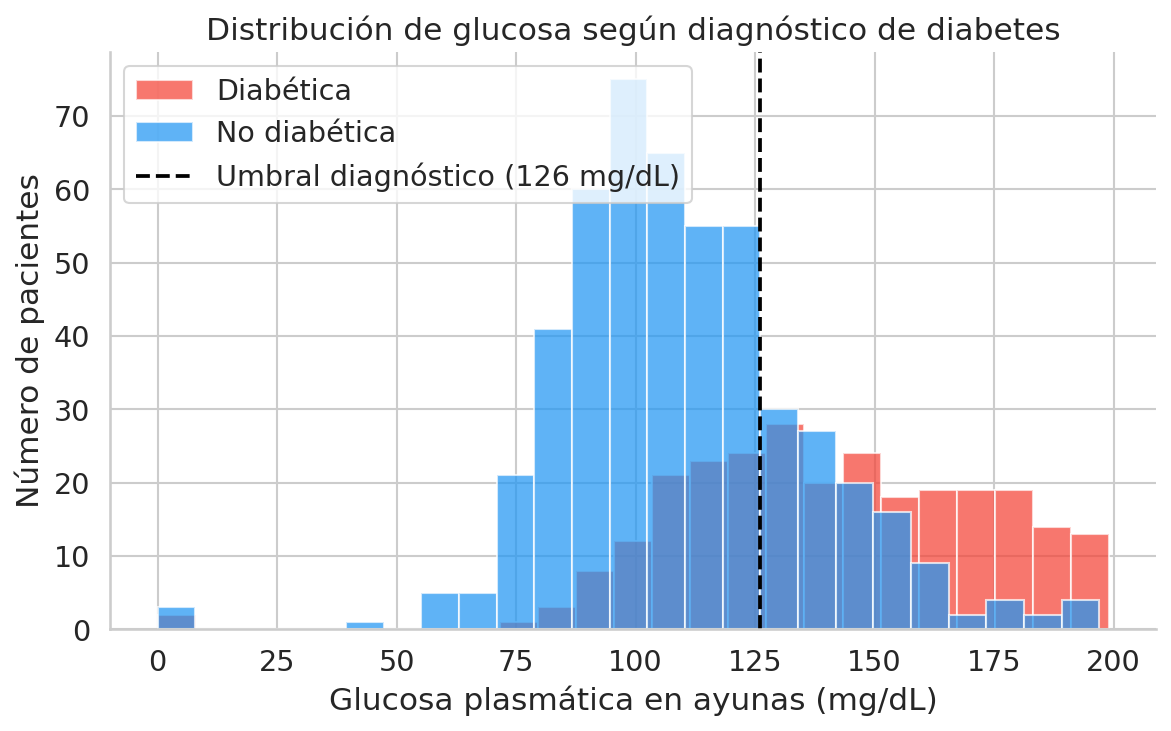
\includegraphics[width=\textwidth]{plots/01_diabetes_glucosa_histograma.png}
        \end{figure}
      \end{block}
    \end{column}
    \begin{column}{0.41\textwidth}
      \vspace{4mm}
      \begin{block}{Anatomía del histograma}
        \begin{itemize}\small
          \item \textbf{Eje X}: valores de la variable
          \item \textbf{Eje Y}: frecuencia (o densidad)
          \item \textbf{Forma}: simétrica, sesgada, bimodal
          \item \textbf{Cola}: dónde están los extremos
        \end{itemize}
      \end{block}
      \vspace{4mm}
      \begin{exampleblock}{Por qué importa}
        \scriptsize Estancias UCI: \{1, 2, 3, 4, 120\} días.\\[1mm]
        Media\,=\,26 días\\
        Mediana\,=\,3 días\\[2mm]
        La media no representa al paciente típico.\\
        La asimetría la veis en el histograma\\
        antes de calcular nada.
      \end{exampleblock}
    \end{column}
  \end{columns}
\end{frame}

% SLIDE 32 - Boxplot comparar grupos --------------------------------------------------
\begin{frame}{Boxplot --- Comparar grupos}
  \begin{columns}[T]
    \begin{column}{0.52\textwidth}
      \begin{block}{Marcador hormonal --- Tumor neuroendocrino (n\,=\,493)}
        \begin{figure}[H]
          \centering
          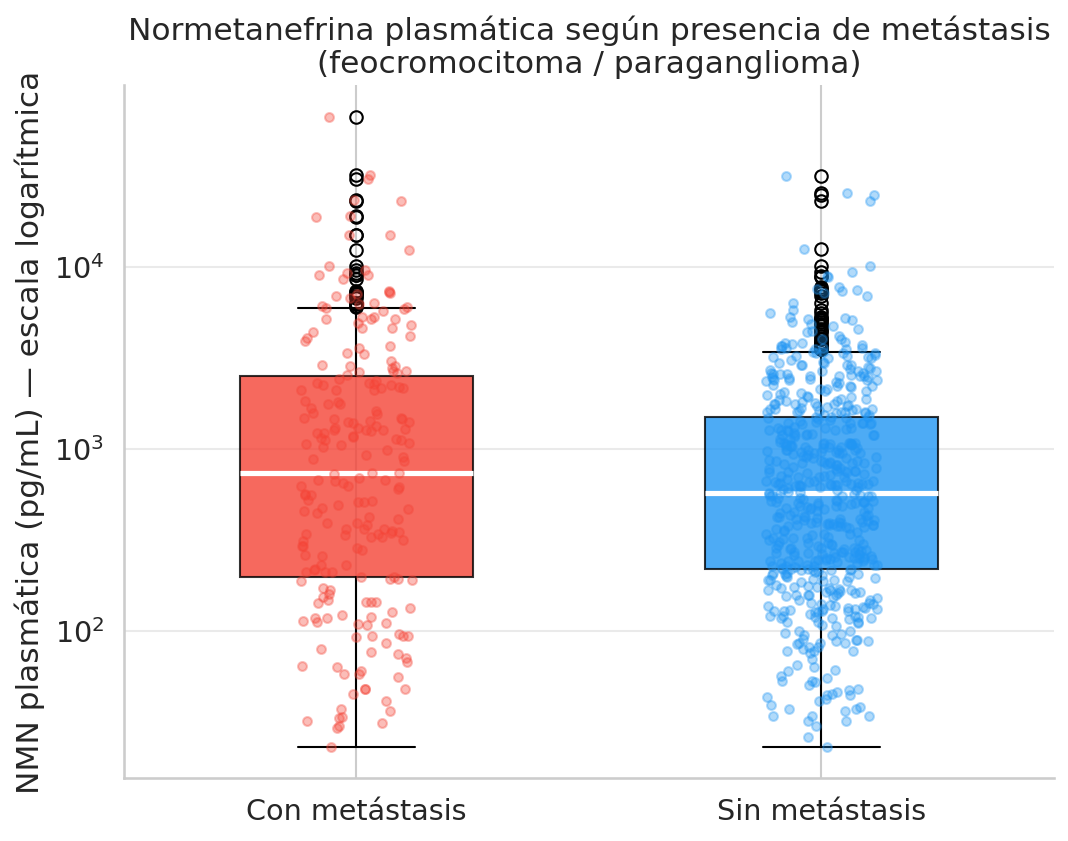
\includegraphics[width=\textwidth]{plots/06_metastasis_nmn_boxplot.png}
        \end{figure}
      \end{block}
    \end{column}
    \begin{column}{0.45\textwidth}
      \vspace{2mm}
      \begin{block}{Anatomía del boxplot}
        \centering
        \begin{tikzpicture}[scale=0.75,transform shape]
          \draw[thick,UCblue] (0.8,1.0) rectangle (3.2,3.0);
          \draw[UCred,line width=2pt] (0.8,2.1) -- (3.2,2.1);
          \draw[thick,UCblue] (2.0,1.0) -- (2.0,0.2);
          \draw[thick,UCblue] (2.0,3.0) -- (2.0,3.8);
          \draw[thick,UCblue] (1.4,0.2) -- (2.6,0.2);
          \draw[thick,UCblue] (1.4,3.8) -- (2.6,3.8);
          \fill[UCred] (2,4.5) circle (2.5pt);
          \node[right,font=\tiny,UCred]  at (3.35,2.1) {mediana};
          \node[right,font=\tiny,UCblue] at (3.35,1.0) {P25};
          \node[right,font=\tiny,UCblue] at (3.35,3.0) {P75};
          \node[right,font=\tiny,UCgray] at (3.35,0.2) {mín};
          \node[right,font=\tiny,UCgray] at (3.35,3.8) {máx};
          \node[right,font=\tiny,UCred]  at (3.35,4.5) {outlier};
          \draw[<->,UCgray,thin] (0.3,1.0) -- (0.3,3.0)
            node[midway,left,font=\tiny] {IQR};
        \end{tikzpicture}
      \end{block}
      \vspace{2mm}
      {\scriptsize Nivel bajo (sin riesgo) vs.\ alto (con riesgo).\\
      Sin ningún test: el gráfico ya habla.}
    \end{column}
  \end{columns}
\end{frame}

% SLIDE 33 - Scatter dos biomarcadores --------------------------------------------
\begin{frame}{Scatter plot --- Relación entre dos variables}
  \begin{columns}[T]
    \begin{column}{0.52\textwidth}
      \begin{block}{Dos biomarcadores --- dos grupos clínicos}
        \begin{figure}[H]
          \centering
          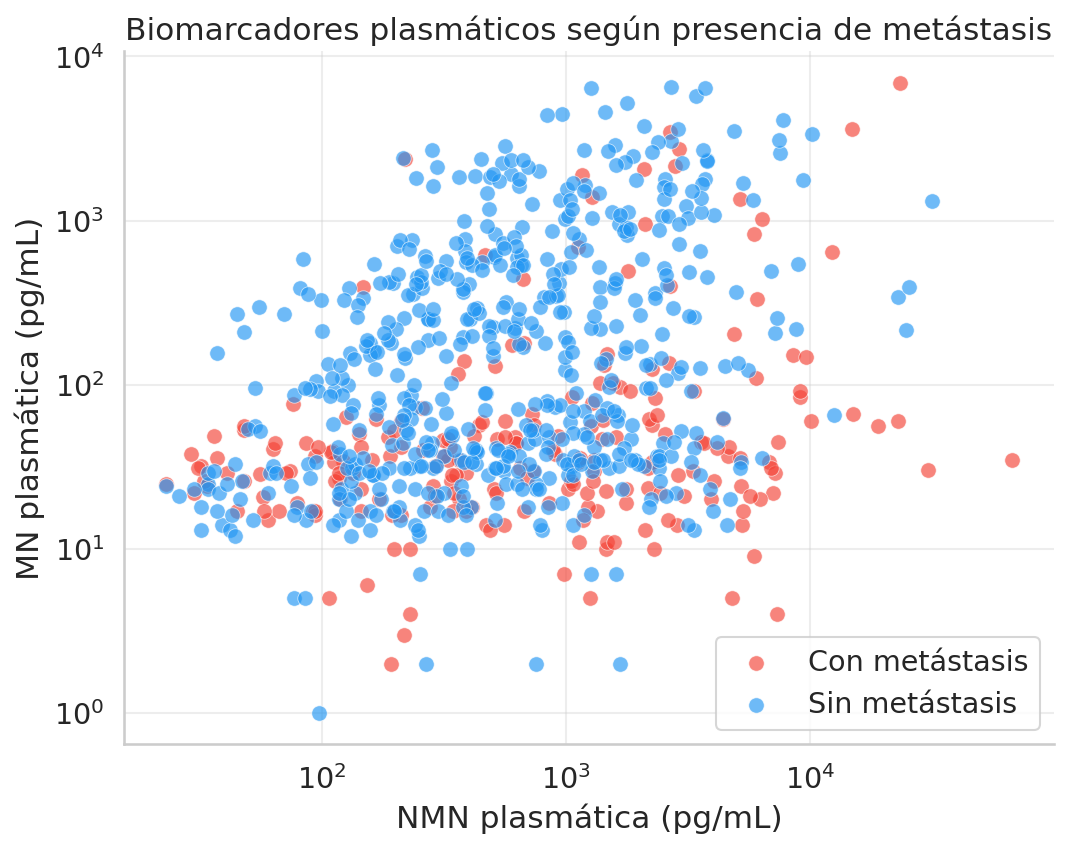
\includegraphics[width=\textwidth]{plots/07_metastasis_nmn_mn_scatter.png}
        \end{figure}
      \end{block}
    \end{column}
    \begin{column}{0.45\textwidth}
      \vspace{4mm}
      \begin{block}{Qué buscar}
        \begin{itemize}\small
          \item Cada punto = un paciente
          \item Color = grupo clínico (riesgo bajo / alto)
          \item Patrón en nube = correlación
          \item Grupos separados = clasificación posible
          \item Outliers visibles inmediatamente
        \end{itemize}
      \end{block}
      \vspace{4mm}
      \begin{exampleblock}{}
        \small La separación visual entre grupos informa\\
        sobre la viabilidad de un modelo.\\[2mm]
        \scriptsize El scatter orienta antes de ajustar nada.
      \end{exampleblock}
    \end{column}
  \end{columns}
\end{frame}

% SLIDE 34 - Curva ROC -----------------------------------------------------
\begin{frame}{Curva ROC --- Capacidad discriminativa}
  \begin{columns}[T]
    \begin{column}{0.48\textwidth}
      \begin{block}{Regresión logística, Diabetes Pima}
        \begin{figure}[H]
          \centering
          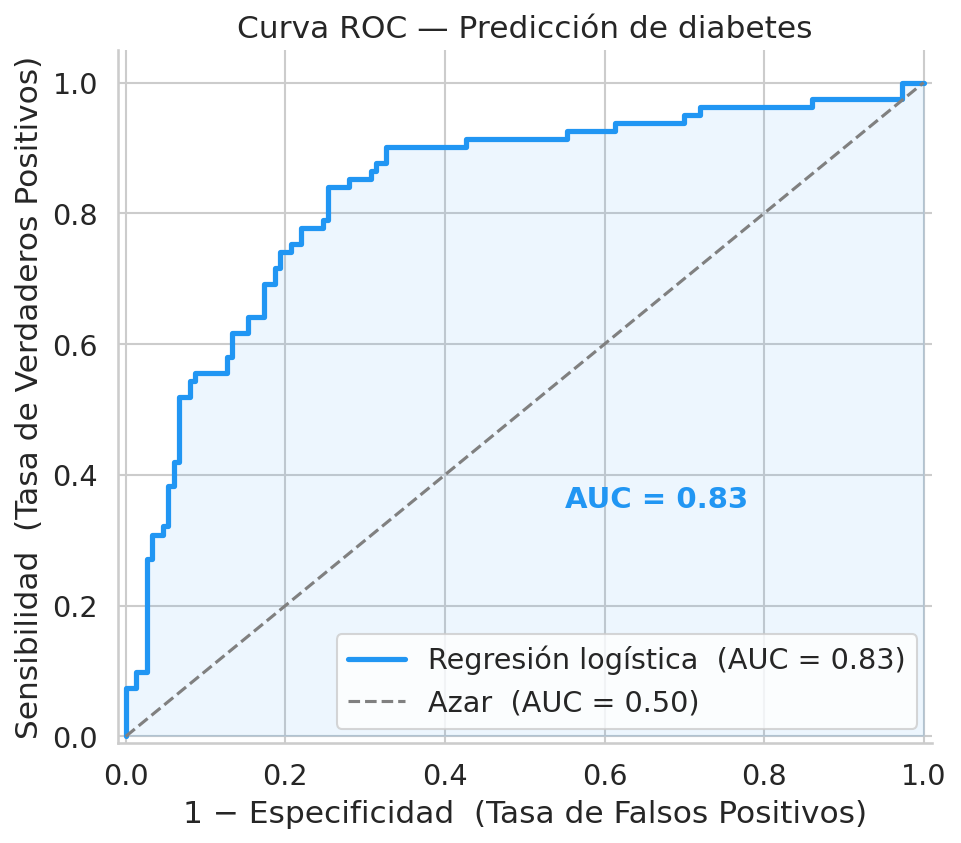
\includegraphics[width=\textwidth]{plots/04_diabetes_roc_curve.png}
        \end{figure}
      \end{block}
    \end{column}
    \begin{column}{0.48\textwidth}
      \begin{block}{Guía de interpretación del AUC}
        \begin{figure}[H]
          \centering
          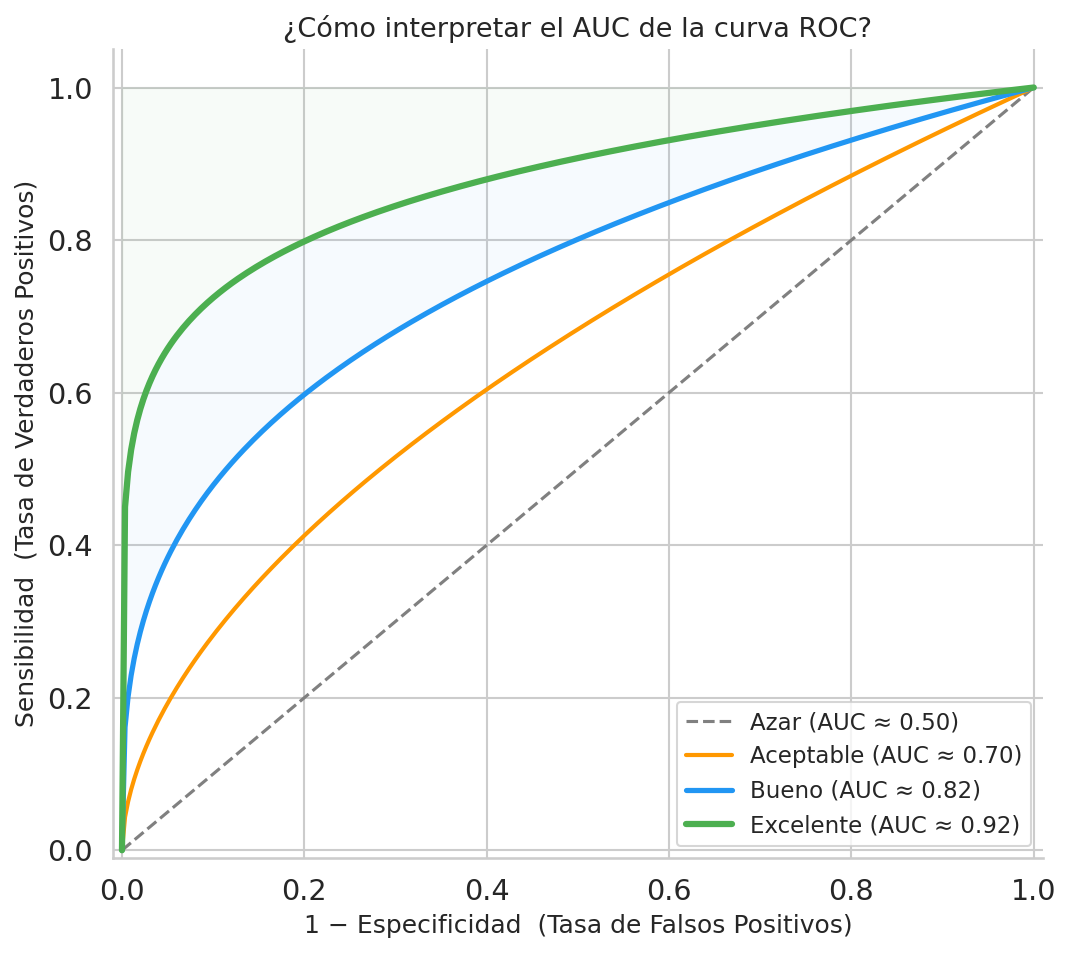
\includegraphics[width=\textwidth]{plots/15_guia_interpretacion_auc.png}
        \end{figure}
      \end{block}
    \end{column}
  \end{columns}
  \vspace{2mm}
  \begin{columns}[T]
    \begin{column}{0.50\textwidth}
      \begin{exampleblock}{AUC --- Área Under the Curve}
        \renewcommand{\arraystretch}{1.2}
        \scriptsize\centering
        \begin{tabular}{lc}
          \toprule
          AUC & Interpretación \\
          \midrule
          0{,}5        & Azar \\
          0{,}6--0{,}7 & Discriminación pobre \\
          0{,}7--0{,}8 & Aceptable \\
          0{,}8--0{,}9 & Buena \\
          $>0{,}9$     & Excelente \\
          \bottomrule
        \end{tabular}
      \end{exampleblock}
    \end{column}
    \begin{column}{0.47\textwidth}
      \begin{block}{}
        \scriptsize
        Eje X: Falsos positivos (1\,--\,Especificidad)\\[1mm]
        Eje Y: Verdaderos positivos (Sensibilidad)\\[1mm]
        Diagonal = azar puro \quad
        Esquina sup.\ izq. = perfecto\\[2mm]
        Útil para cualquier biomarcador o escala clínica,\\
        no solo para modelos de ML.
      \end{block}
    \end{column}
  \end{columns}
\end{frame}

% SLIDE 35 - El descriptivo informa el modelo ---------------------------------------
\begin{frame}{El descriptivo informa el modelo}
  \begin{columns}[T]
    \begin{column}{0.52\textwidth}
      \begin{block}{Árbol de decisión --- Diabetes Pima}
        \begin{figure}[H]
          \centering
          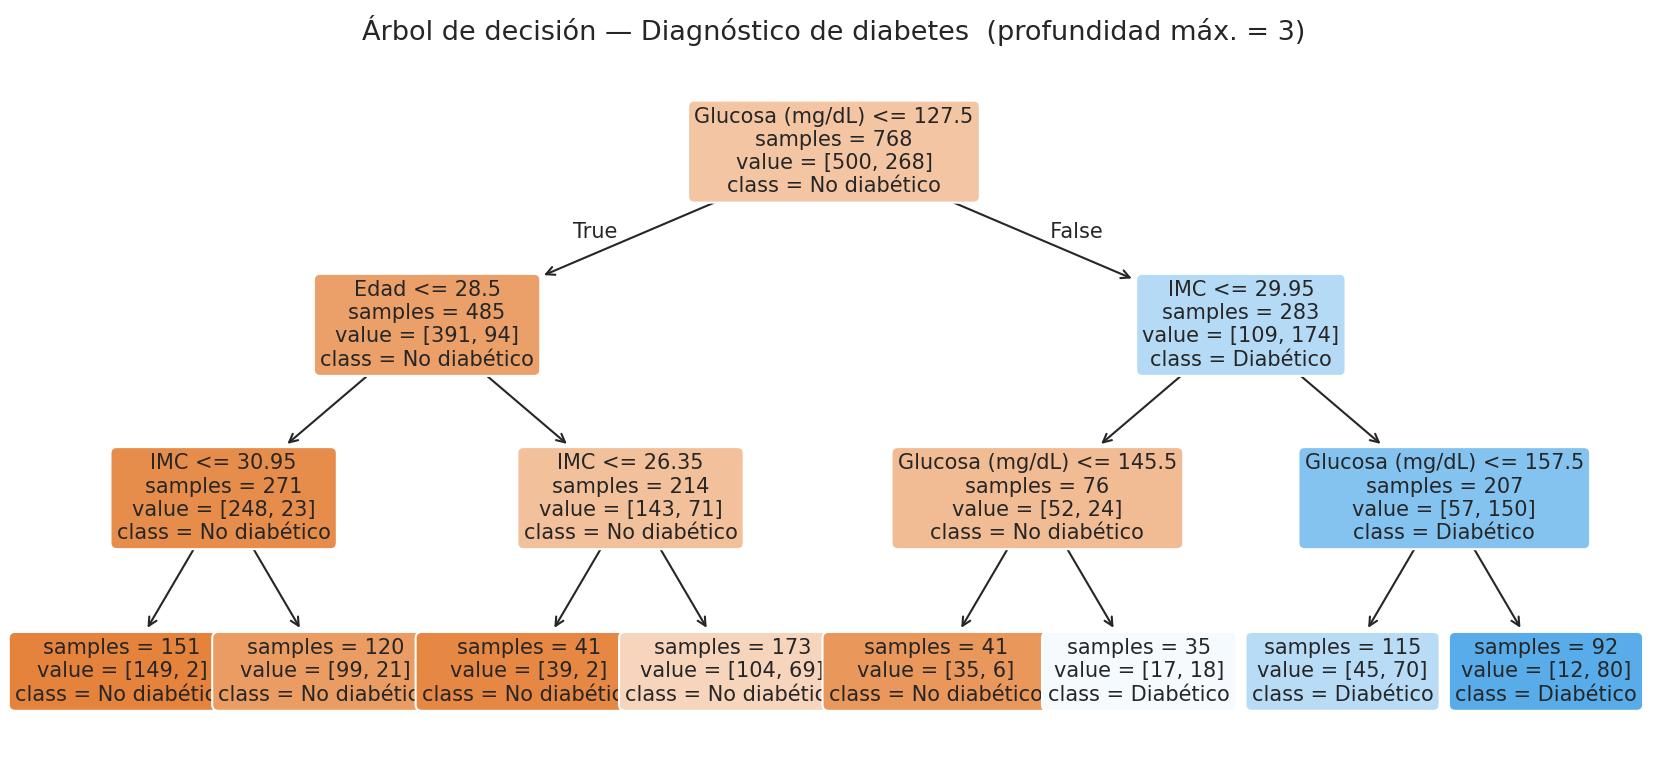
\includegraphics[width=\textwidth]{plots/05_diabetes_arbol_decision.png}
        \end{figure}
      \end{block}
    \end{column}
    \begin{column}{0.45\textwidth}
      \vspace{4mm}
      \begin{block}{El descriptivo como base}
        \begin{itemize}\small
          \item Los splits del árbol reflejan la separación\\
                que ya visteis en histogramas y boxplots
          \item Si las distribuciones se solapan,\\
                el modelo tampoco separará
          \item El descriptivo \textbf{predice la calidad}\\
                del modelo antes de entrenarlo
        \end{itemize}
      \end{block}
      \vspace{4mm}
      \begin{exampleblock}{}
        \small El análisis descriptivo no es un preámbulo.\\[2mm]
        \textbf{Es la base sobre la que se construye\\
        cualquier modelo posterior.}
      \end{exampleblock}
    \end{column}
  \end{columns}
  \note{No entrar en detalles del árbol. Es para mostrar que el trabajo descriptivo previo explica y limita lo que el modelo puede lograr.}
\end{frame}

% SLIDE 36 - Kaplan-Meier --------------------------------------------------
\begin{frame}{Curva de Kaplan-Meier --- Para cuando trabajáis con tiempo}
  \begin{columns}[T]
    \begin{column}{0.52\textwidth}
      \begin{block}{Cómo se lee una curva KM}
        \centering\vspace{3mm}
        \begin{tikzpicture}[scale=0.80,transform shape]
          \draw[->,thick,UCgray] (0,0) -- (0,4.0)
            node[above,font=\tiny] {Supervivencia};
          \draw[->,thick,UCgray] (0,0) -- (6.5,0)
            node[right,font=\tiny] {Tiempo};
          \foreach \v/\y in {1.0/3.6,0.75/2.7,0.50/1.8,0.25/0.9}{
            \draw[UCgray,thin] (-0.08,\y) -- (0.08,\y);
            \node[left,font=\tiny,UCgray] at (-0.1,\y) {\v};
          }
          \draw[UCblue,very thick]
            (0,3.6) -- (1,3.6) -- (1,3.2)
            -- (2,3.2) -- (2,2.9)
            -- (3,2.9) -- (3,2.5)
            -- (4.5,2.5) -- (4.5,2.1)
            -- (6,2.1);
          \node[right,font=\tiny,UCblue] at (6.1,2.1) {Tratam.};
          \draw[UCred,very thick]
            (0,3.6) -- (0.6,3.6) -- (0.6,2.9)
            -- (1.2,2.9) -- (1.2,2.3)
            -- (2.0,2.3) -- (2.0,1.7)
            -- (3.0,1.7) -- (3.0,1.1)
            -- (4.0,1.1) -- (4.0,0.5)
            -- (6,0.5);
          \node[right,font=\tiny,UCred] at (6.1,0.5) {Control};
          \draw[<-,UCgray,thin] (1,3.4) -- (1.6,3.9)
            node[right,font=\tiny,UCgray] {escalón\,=\,evento};
        \end{tikzpicture}
      \end{block}
    \end{column}
    \begin{column}{0.45\textwidth}
      \vspace{3mm}
      \begin{itemize}\small
        \item \textbf{Escalón} hacia abajo = un evento
        \item \textbf{Separación} entre curvas = diferencia entre grupos
        \item El $p$-valor del paper confirma si esa diferencia es significativa
        \item La curva que desciende más rápido = peor pronóstico
      \end{itemize}
    \end{column}
  \end{columns}
\end{frame}

% SLIDE 37 - Eleccion del grafico ------------------------------------------
\begin{frame}{Cómo elegir el gráfico correcto}
  \begin{center}
    \renewcommand{\arraystretch}{1.5}
    \begin{tabular}{p{3.0cm} p{3.0cm} p{2.8cm} p{3.5cm}}
      \toprule
      \textbf{Pregunta} & \textbf{Variable} & \textbf{Grupos} & \textbf{Gráfico} \\
      \midrule
      ¿Cómo se distribuye? & Continua      & 1    & Histograma \\
      ¿Hay diferencia?     & Continua      & 2--3 & Boxplot \\
      ¿Hay relación?       & 2 continuas   & ---  & Scatter \\
      ¿Qué proporción?     & Categórica    & ---  & Barras horiz. \\
      ¿Muchas variables?   & Continuas     & ---  & Heatmap \\
      ¿Tiempo a evento?    & Supervivencia & 2+   & Kaplan-Meier \\
      \bottomrule
    \end{tabular}
  \end{center}
\end{frame}

% SLIDE 38 - Mensaje clave visualizacion -----------------------------------
\begin{frame}
  \begin{center}
    \vspace{4mm}
    {\color{UCblue!30}\rule{\textwidth}{1.5pt}}
    \vspace{6mm}
    \begin{beamercolorbox}[sep=18pt,center,rounded=true,shadow=true]{block title example}
      \LARGE\bfseries Un buen gráfico no es decoración.\\[4mm]
      \Large Es información comprimida.
    \end{beamercolorbox}
    \vspace{6mm}
    {\color{UCblue!30}\rule{\textwidth}{1.5pt}}
  \end{center}
\end{frame}


% =========================================================================
\section{Cierre}
% =========================================================================

% SLIDE 39 - Pipeline de trabajo ------------------------------------------
\begin{frame}{Flujo de trabajo en la práctica}
  \centering
  \begin{tikzpicture}[scale=0.76,transform shape,node distance=0.1cm]
    \tikzset{paso/.style={rectangle,draw=UCblue,fill=UCbluePale,
             minimum width=2.0cm,minimum height=1.0cm,text centered,
             font=\scriptsize,rounded corners=0.12cm,text width=1.9cm}}
    \tikzset{pasog/.style={paso,fill=UCgreen!18,draw=UCgreen}}
    \tikzset{pasor/.style={paso,fill=UCred!10,draw=UCred!70}}
    \node[paso]  (p1) at (0,0)    {1. Definir la pregunta};
    \node[paso]  (p2) at (2.5,0)  {2. Libro de códigos};
    \node[pasor] (p3) at (5.0,0)  {3. Inspección de datos};
    \node[pasor] (p4) at (7.5,0)  {4. Limpieza / imputación};
    \node[pasog] (p5) at (5.0,-2) {5. Análisis descriptivo};
    \node[pasog] (p6) at (2.5,-2) {6. Table 1};
    \node[pasog] (p7) at (0.0,-2) {7. Visualización};
    \node[paso]  (p8) at (7.5,-2) {8. Hipótesis / modelo};
    \draw[->,thick,UCblue!70] (p1.east) -- (p2.west);
    \draw[->,thick,UCblue!70] (p2.east) -- (p3.west);
    \draw[->,thick,UCblue!70] (p3.east) -- (p4.west);
    \draw[->,thick,UCblue!70] (p4.south) -- (p4.south |- p5.north) -- (p5.north);
    \draw[->,thick,UCgreen!70](p5.west)  -- (p6.east);
    \draw[->,thick,UCgreen!70](p6.west)  -- (p7.east);
    \draw[->,thick,UCblue!70] (p5.east)  -- (p8.west);
    \node[font=\tiny,UCred,below] at (5.0,-0.6)
      {Donde se produce el 80\,\% de los problemas};
  \end{tikzpicture}
  \vspace{4mm}
  \begin{columns}[T]
    \begin{column}{0.48\textwidth}
      \begin{block}{}
        \scriptsize Los pasos 3 y 4 se suelen saltar.\\
        Son los que más impactan en la calidad del análisis.
      \end{block}
    \end{column}
    \begin{column}{0.48\textwidth}
      \begin{exampleblock}{}
        \scriptsize El paso 1 (la pregunta) se suele hacer mal.\\
        Definidla antes de abrir cualquier archivo.
      \end{exampleblock}
    \end{column}
  \end{columns}
\end{frame}

% SLIDE 40 - Limitaciones --------------------------------------------------
\begin{frame}{Limitaciones del análisis descriptivo}
  \begin{columns}[T]
    \begin{column}{0.50\textwidth}
      \begin{block}{Lo que el descriptivo NO puede hacer}
        \begin{itemize}\small
          \item \no\ Establecer causalidad
          \item \no\ Generalizar más allá de la muestra
          \item \no\ Reemplazar el criterio clínico
          \item \no\ Compensar un sesgo de selección grave
        \end{itemize}
      \end{block}
    \end{column}
    \begin{column}{0.47\textwidth}
      \vspace{3mm}
      \begin{exampleblock}{Buenas prácticas}
        \begin{enumerate}\small
          \item Definir la hipótesis \textbf{antes} de ver los datos
          \item Documentar cada decisión de limpieza
          \item Reportar missings y exclusiones
          \item Distinguir exploración de confirmación
        \end{enumerate}
      \end{exampleblock}
    \end{column}
  \end{columns}
\end{frame}

% SLIDE 41 - Los 3 mandamientos -------------------------------------------
\begin{frame}{Los 3 mandamientos del análisis descriptivo}
  \begin{center}
    \vspace{5mm}
    \begin{beamercolorbox}[sep=12pt,center,rounded=true,shadow=true]{block title}
      \large\bfseries I.\quad Define el \textit{outcome} \textbf{antes} de abrir el Excel.
    \end{beamercolorbox}
    \vspace{5mm}
    \begin{beamercolorbox}[sep=12pt,center,rounded=true,shadow=true]{block title}
      \large\bfseries II.\quad Revisa los missings antes de ejecutar cualquier análisis.
    \end{beamercolorbox}
    \vspace{5mm}
    \begin{beamercolorbox}[sep=12pt,center,rounded=true,shadow=true]{block title}
      \large\bfseries III.\quad El Table~1 bien hecho \textbf{ya es un resultado.}
    \end{beamercolorbox}
  \end{center}
  \note{Leer cada uno con pausa de 3 segundos.}
\end{frame}

% SLIDE 42 - Slide final --------------------------------------------------
\begin{frame}
  \begin{center}
    \vspace{6mm}
    {\LARGE Los médicos con datos bien analizados}\\[3mm]
    {\LARGE ya hacen ciencia clínica.}
    \vspace{6mm}\\
    {\large No necesitáis empezar por el machine learning para publicar.}\\[3mm]
    {\large Necesitáis una pregunta bien formulada,}\\[2mm]
    {\large datos bien recogidos,}\\[2mm]
    {\large y herramientas para contarle la historia a los revisores.}
  \end{center}
\end{frame}

% SLIDE 43 - Portada final ------------------------------------------------
\begin{frame}
  \titlepage
\end{frame}

\end{document}